Following the Introduction's exploration of AI's emerging role in software architecture, this Literature Review aims to deepen our understanding. It sets out to map the current landscape of AI advancements and software pattern methodologies, framing the context for our research. 

The chapter provides a thorough overview of two key areas: the evolution of AI, particularly \ac{LLM} and Prompt Engineering, and the selection methods of software patterns. This review will underpin our investigation into AI-assisted tools for design decision-making in software projects.

\MyParaBold{Chapter Overview}
\begin{itemize}
    \item \textbf{Evolution of AI and Large Language Models:} Examines how AI has evolved, focusing on large language models and their impact on software development.

    \item \textbf{Prompt Engineering in AI:} Discusses prompt engineering principles and their applications in software development.

    \item \textbf{Tools for Developers:} Reviews current AI tools for software development. 

    \item \textbf{Software Patterns and Design Pattern Selection Methods:} Traces the history of software patterns and analyzes methods for selecting design patterns, setting the stage for our AI-focused exploration in subsequent chapters.
\end{itemize}


\section{An Overview of the Evolution of AI}\label{sec:AI-evolution}
\ac{AI} is a broad field encompassing the study and creation of systems that can perform tasks that usually require human intelligence, such as reasoning, learning, perception, and decision-making. The term was coined by John McCarthy in 1956, who defined it as "the science and engineering of making intelligent machines." \cite{Mccarthy2006}. Since then, AI has evolved into various sub-fields and paradigms, such as symbolic AI, connectionism, evolutionary computation, and machine learning. 

\ac{ML} is a subset of AI that uses data and algorithms to allow systems to learn and improve from experience without being explicitly programmed~\cite{Mitchell2007}. This concept can be applied in several domains, such as computer vision, speech recognition, natural language processing, bioinformatics, recommendation and virtual assistants. For example, Alexa\footnote{\url{https://www.amazon.com/alexa}} , Google Assistant\footnote{\url{https://assistant.google.com}}, Apple Siri\footnote{\url{https://www.apple.com/siri}} are products that use \ac{ML} techniques for understanding and responding to voice commands, providing information, and performing tasks. Another example is Netflix\footnote{\url{https://www.netflix.com}}, which uses \ac{ML} to recommend movies and shows to its users based on their preferences and behavior.

\ac{DL} is a branch of \ac{ML} that uses multi-layered artificial neural networks to learn from large and complex datasets~\cite{LeCun2015}.~\ac{DL} can perform various tasks involving images, text, and audio, such as classification, recognition, generation, and translation. For example,~\ac{DL} can sort animal images into different categories~\cite{Krizhevsky2017}, recognize celebrity faces~\cite{Schroff2015}, generate captions for images~\cite{Vinyals2015}, translate sentences from one language to another~\cite{Sutskever2014}, and synthesize realistic human voices~\cite{Oord2016}. \ac{DL} has also improved domains such as medicine, finance, and entertainment by providing customized solutions, detecting fraud, and creating realistic simulations. For example, \ac{DL} can diagnose skin cancer from images of skin lesions~\cite{Esteva2017}, identify credit card fraud from transaction data~\cite{Awoyemi2017}, create human-like agents for games~\cite{Silver2017}, and generate photorealistic faces of non-existent people~\cite{Karras2019}.

\ac{NLP} is a subfield of~\ac{AI} that deals with the interaction between computers and human languages.~\ac{NLP} aims to enable systems to understand, analyze, generate, and manipulate natural language texts and speech. NLP has many applications in various domains~\cite{Devlin2018}, such as information retrieval, sentiment analysis, summarization, dialogue systems, chatbots, and natural language understanding.~\ac{NLP} also involves studying the linguistic and cognitive aspects of human language processing and communication.

\subsection{Large Language Models}\label{sec:llm}

\ac{LLM} is a type of~\ac{DL} model that can perform various natural language processing tasks, such as generating and classifying text, answering questions conversationally, and translating text from one language to another. \ac{LLM} are trained on massive amounts of unlabeled text using self-supervised or semi-supervised learning. They learn to predict the next token in a sequence given the previous context~\cite{Ozdemir2023}. The term "large" refers to the number of parameters or weights the model can adjust during training, ranging from millions to trillions. \ac{LLM} are general-purpose models that can adapt to different domains and tasks with minimal supervision.

Transformers are a type of neural network architecture and, therefore, a type of \ac{DL}, as shown in Figure~\ref{fig-transformers} representing a set of nested AI technologies leading up to transformers, which became the dominant approach for building LLMs and other NLP models, this is a way to address the limitations of~\ac{RRN} and~\ac{CNN}s for sequence modeling tasks and allows the model to focus on different parts of the input and output strings depending on the context~\cite{Vaswani2017} bringing significant improvements in various~\ac{NLP} tasks such as machine translation, text summarization, question answering and text generation.

% Start Figure ---------------------------
\begin{figure}[ht]
\caption{A nested set of technologies from AI to transformers.}
\centering
\label{fig-transformers}
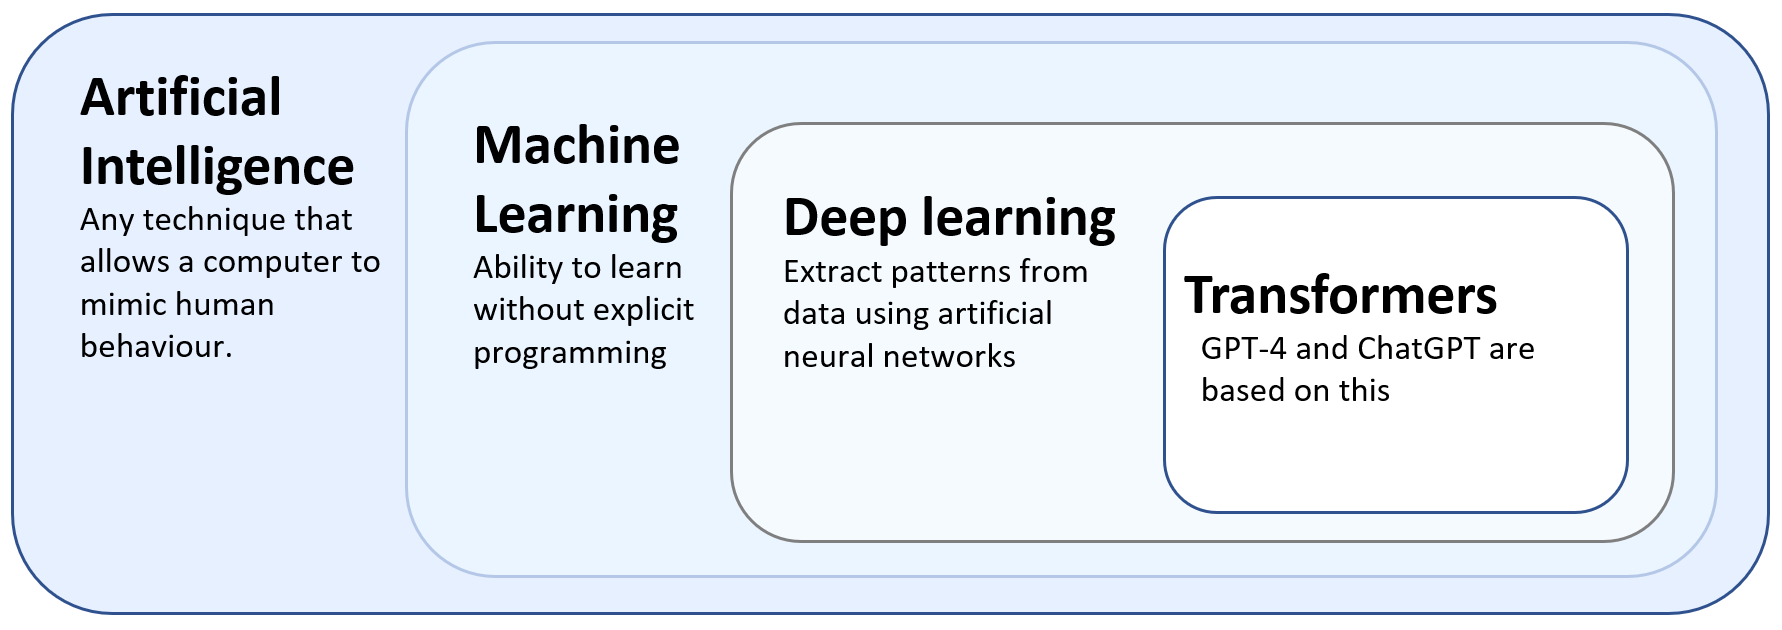
\includegraphics[width=.95\textwidth]{figures/transformers.png}
\objectsource{\textcite{Olivier2024}}
\end{figure}
% End Figure ---------------------------

As~\ac{AI} progresses, ethical concerns about privacy, bias, and liability are becoming increasingly significant ~\cite{Floridi2022}. This is especially true for large language models like GPT-4, which can generate coherent and diverse text based on a given prompt~\cite{Brown2020}. These models present challenges, including data leakage, misinformation, intellectual property rights, and responsibility for generated text, as~\cite{Yan2023}) noted. Thus, it is imperative to evaluate the potential benefits~\cite{Bender2021}.

With the advances of LLMs and Transforms~\cite{Olivier2024}, AI-assisted tools can provide valuable insights and support in various tasks such as solution architecture, agile model storytelling, code generation, automated testing, and DevSecOps. They can improve some stages of the development cycle so software developers, engineers, and architects can improve their project design, resulting in faster and more efficient production and improving overall effectiveness.

The shift from a "data-driven" to an "AI-driven" approach to decision-making workflows is inevitable. While data provides valuable information, human processors have limitations due to cognitive biases and the inability to process large volumes of data efficiently~\cite{Colson2019}. By bringing AI into the workflow, organizations can harness the processing power of AI to extract insights from data and make better decisions. AI can handle complex relationships, non-linear patterns, and large data sets, reducing the impact of human biases~\cite{MichaelRoss2021}.

However, it is important to note that humans still have a role in decision-making, especially regarding unstructured data and factors such as vision, strategy, and values, and the need for collaboration between AI and humans to achieve decision-making more assertive. The integration of AI into workflows, explained in Figure~\ref{fig-decision-making}, is the next phase in our evolution and envisions the collaboration of AI tools with human judgment that will result in the emergence of new companies that embrace AI and human contributions from the ground up start.~\cite{Colson2019}
% Start Figure ---------------------------
\begin{figure}[ht]
\caption{A Decision-Making Model combines the power of AI and Human Judgment.}
\centering
\label{fig-decision-making}
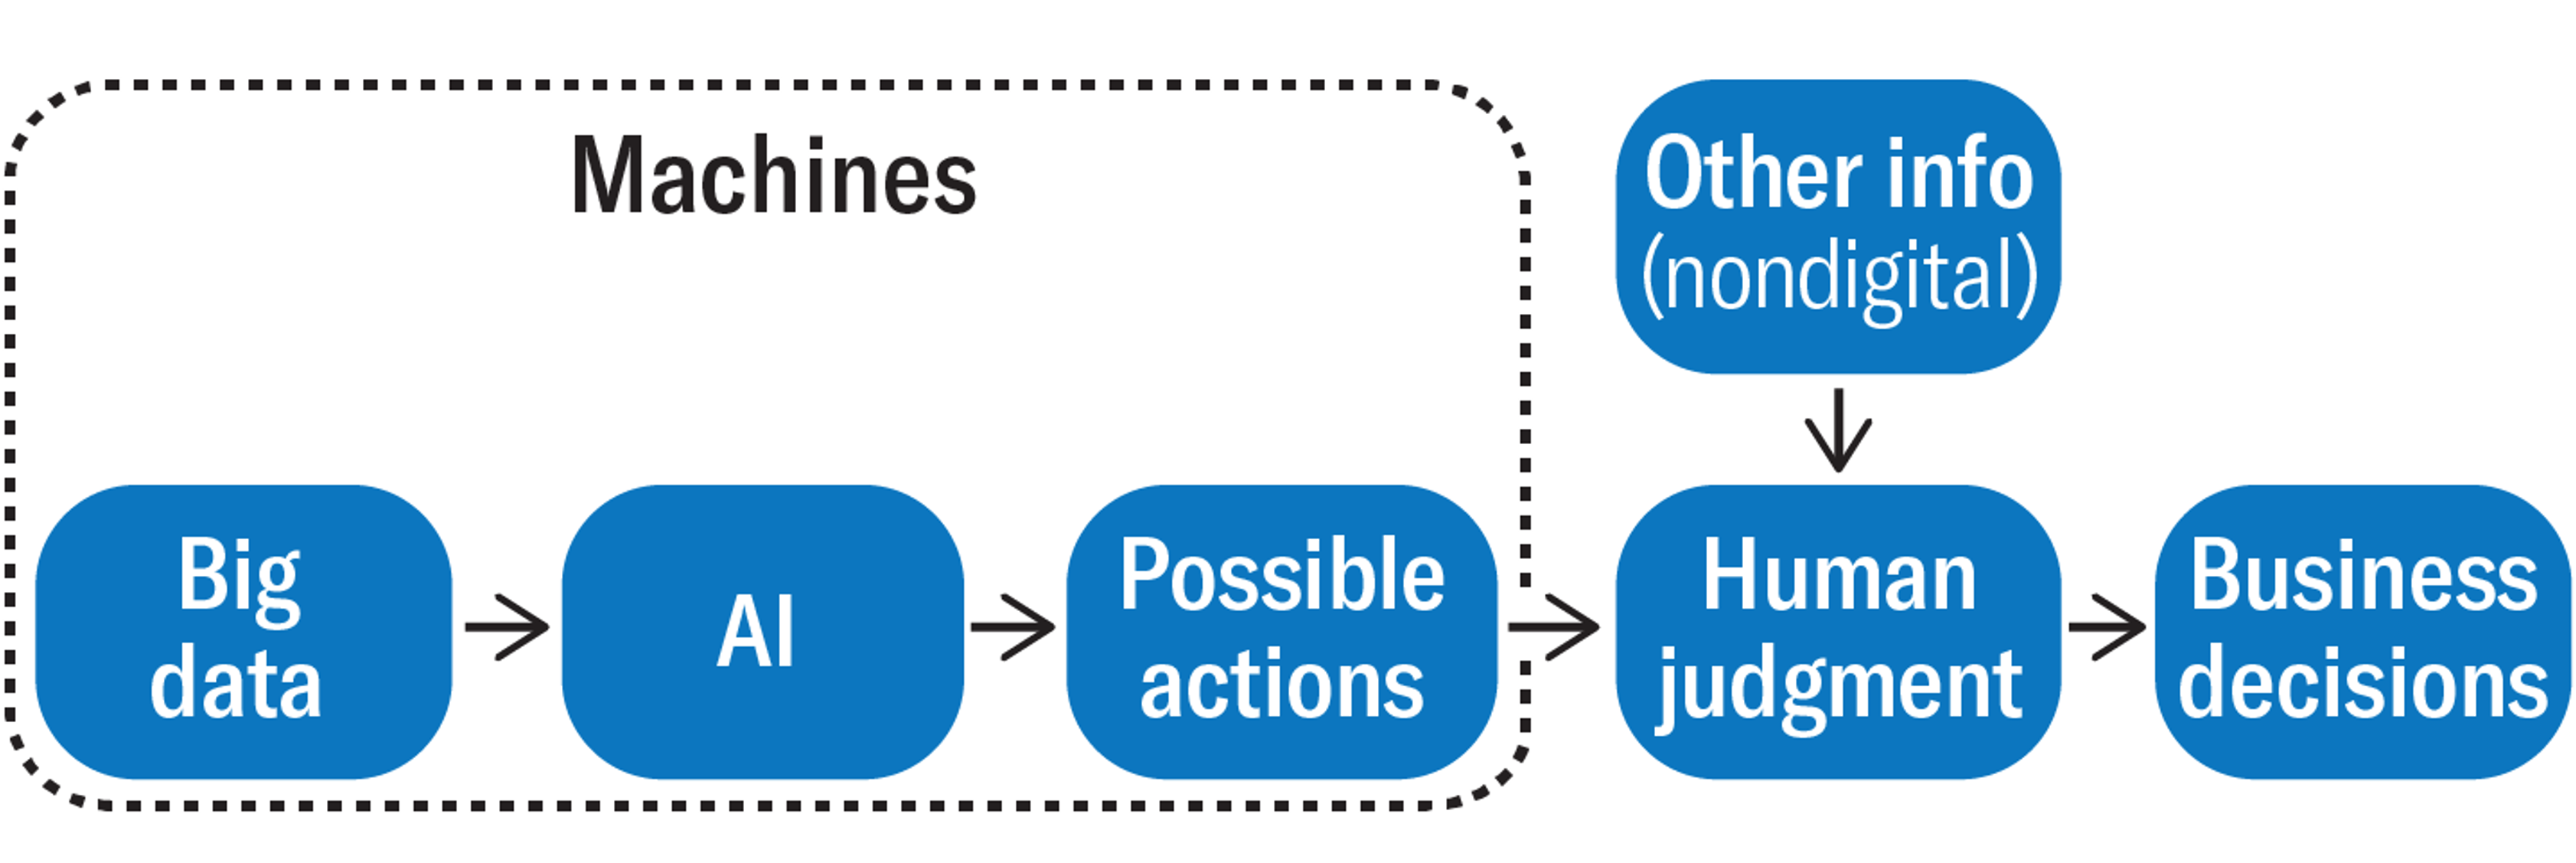
\includegraphics[width=.87\textwidth]{figures/descion-making.png}
\objectsource{\textcite{Colson2019}}
\end{figure}
% End Figure ---------------------------

% \subsection{AI-Assisted Tools in Software Design}\label{sec:AI tools}

\subsection{Prompt Engineering for Generative AI}\label{sec:prompt-engenieer}
Prompt Engineering is critical to interfacing with AI-assisted tools such as GPT-4. Prompts are the starting point of the conversation with the model, acting as an essential guide for the AI's response~\cite{Brown2020}. The AI model generates its response based on the input prompt, with the aim of completing the implied task as accurately as possible.

Prompt Engineering refers to the art and science of crafting effective prompts that can guide the AI model to produce desired and valuable results~\cite{White2023}. An expertly engineered prompt can significantly enhance the performance of an AI tool by narrowing down the scope of potential responses and focusing the AI's "attention" on the relevant aspects of the problem at hand. Therefore, prompt engineering is crucial to using AI tools to solve specific problems.

In software design, prompt engineering becomes particularly significant. Crafting a well-structured prompt that accurately encapsulates the design problem can guide the AI tool to suggest an appropriate design pattern. This not only saves time and effort for developers but also helps to ensure that the resulting software design is robust and efficient.

It's important to note that there is no one-size-fits-all solution when it comes to engineering solutions quickly. Different situations may call for different requests in order to achieve the best possible results. To construct effective prompts, there are five key principles to keep in mind. These principles, known as the "Five Principles of Prompting,"~\cite{Phoenix2024} are as follows:

\begin{enumerate}
    \item \textbf{Giving Direction}: Providing clear instructions and details about your expectations can lead to output that better matches your vision. This is similar to briefing a human co-worker on a task—without adequate context, even the most intelligent AI may struggle to deliver satisfactory results.
    
     \item \textbf{Specifying Format}: Clearly defining the required response format minimizes the potential for parsing errors and reduces the time spent refining the generated output.
    
     \item \textbf{Providing Examples}: Including examples in prompts can guide the AI in understanding the context, thereby enhancing the reliability and accuracy of the output.
    
     \item \textbf{Evaluating Quality}: Identifying and understanding errors can facilitate iterative improvements, enhancing the reliability of generated responses over time.
    
     \item \textbf{Dividing Labor}: It's important to recognize that different models and prompts may be better suited for different tasks. Chaining together multiple models with well-structured prompts can accomplish more sophisticated tasks. 
\end{enumerate}

\textcite{Olivier2024} propose design prompt effective to create a successful prompt\cite{white2023prompt} is usually divided into three parts: context, task, and role, as shown in Figure \ref{fig-design-prompt-effective}. While not all elements are necessary, a well-constructed prompt with clearly defined parts can significantly improve the result.

% Start Figure ----------------------------
\begin{figure}[ht]
\caption{Design of Prompt Effective.}
\centering
\label{fig-design-prompt-effective}
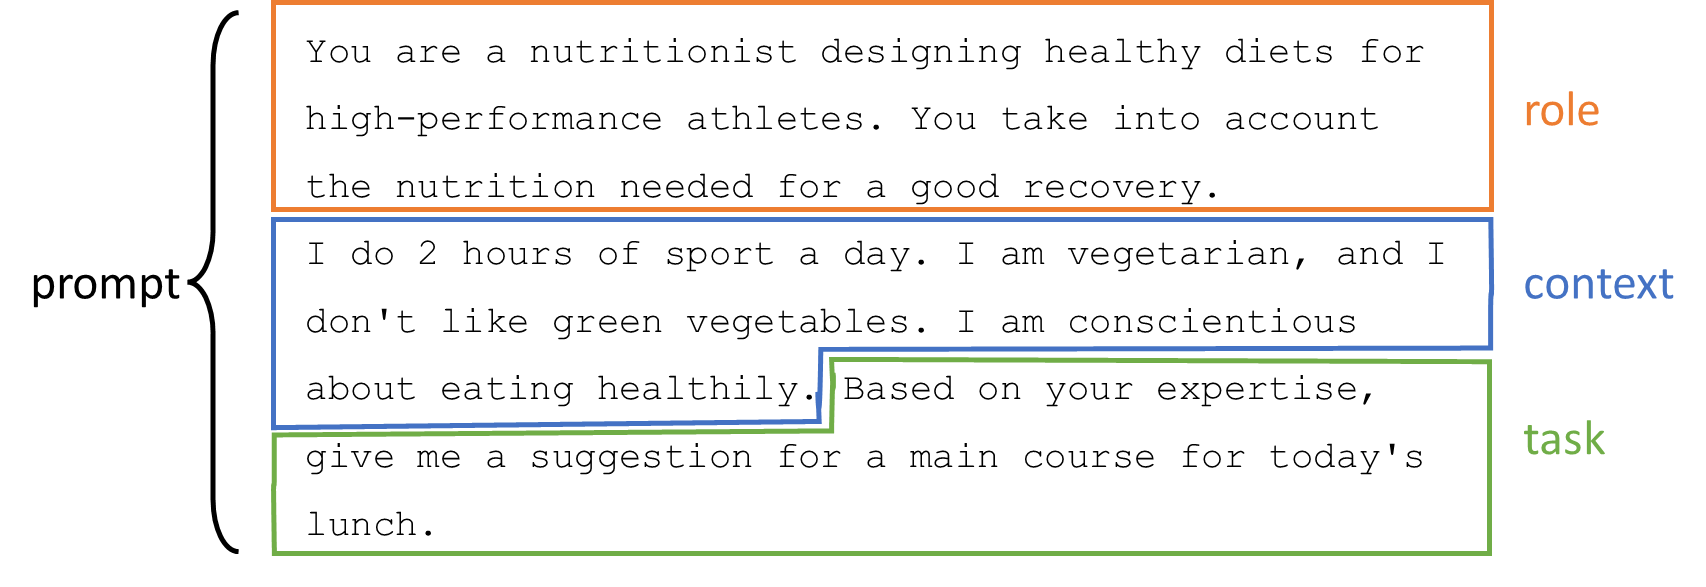
\includegraphics[width=0.9\textwidth]{figures/effetive-prompt.png}
\objectsource{\textcite{Olivier2024}}
\end{figure}
% End Figure ---------------------------

Effective communication skills are key in human and AI interaction. Clearly defined guidelines and expectations can help AI generate creative and unique product names that meet specific criteria. Treat the AI model as a collaborator to maximize its potential in solving complex problems~\cite{Phoenix2024}.
% The potential of these principles and design extends beyond the field of AI. Many of these principles also apply to human collaboration, suggesting that effective communication skills are key in human and AI interaction. For instance, in the context of product naming, clearly defined guidelines and expectations can help the AI generate creative and unique product names that meet specific criteria. By treating the AI model as a collaborator, users can maximize its potential and harness the true power of AI in solving complex problems~\cite{Phoenix2024}.

\MyPara{Few-Shot Learning}

Refers to the ability of the \ac{LLM} to generalize and produce valuable results with only a few examples in the prompt, as illustrated in Figure~\ref{fig-prompt-few-examples}. In the few-shot learning, you give examples of the task you want the model to perform. These examples guide the model to understand the desired output format and the problem-solving process.

% Start Figure ----------------------------
\begin{figure}[ht]
\caption{A prompt containing a few examples}
\centering
\label{fig-prompt-few-examples}
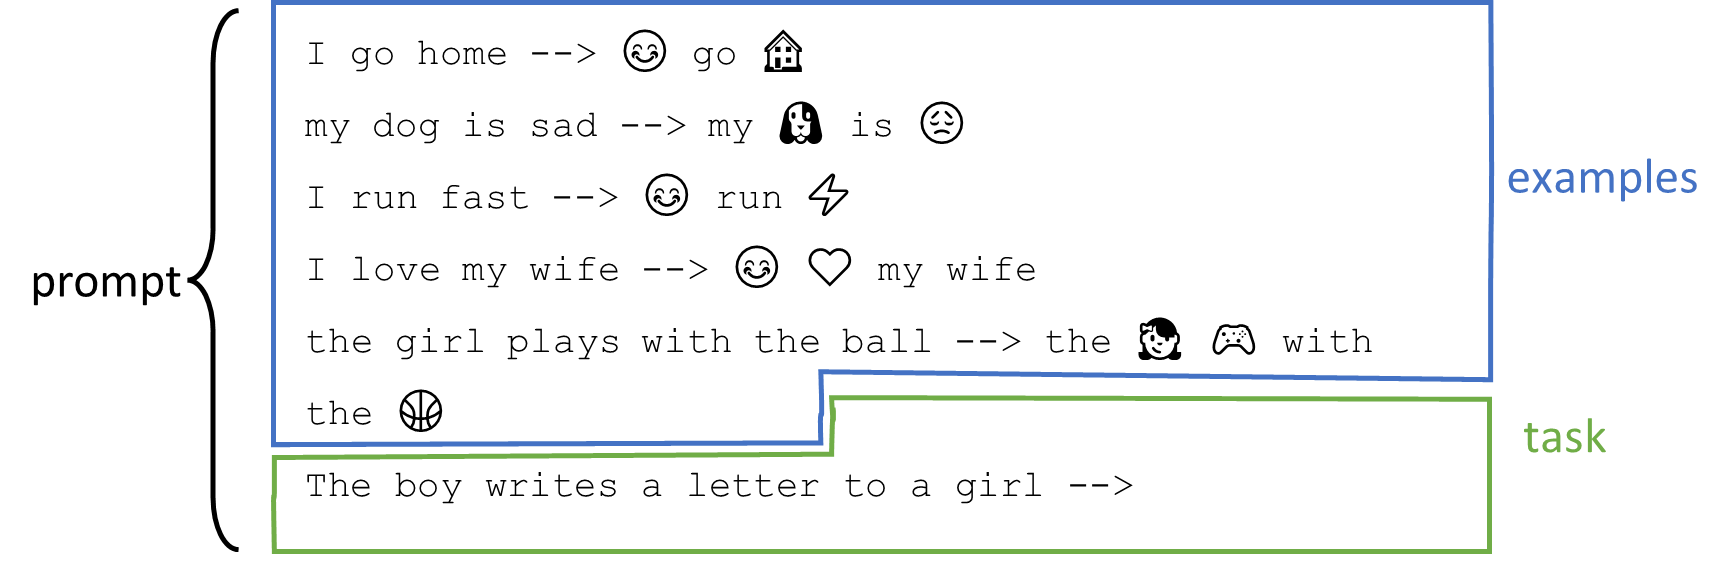
\includegraphics[width=0.9\textwidth]{figures/prompt-few-examples.png}
\objectsource{\textcite{Olivier2024}}
\end{figure}
% End Figure ---------------------------

Consider this example in Figure~\ref{fig-prompt-few-shots-question} of converting certain words into emojis using LLM. It may not be easy to imagine the exact prompt for this task. However, with the help of few-shot learning, the process becomes easier. Provide examples, and the model will attempt to replicate them automatically.

% Start Figure ----------------------------
\begin{figure}[ht]
\caption{A prompt few-shot question}
\centering
\label{fig-prompt-few-shots-question}
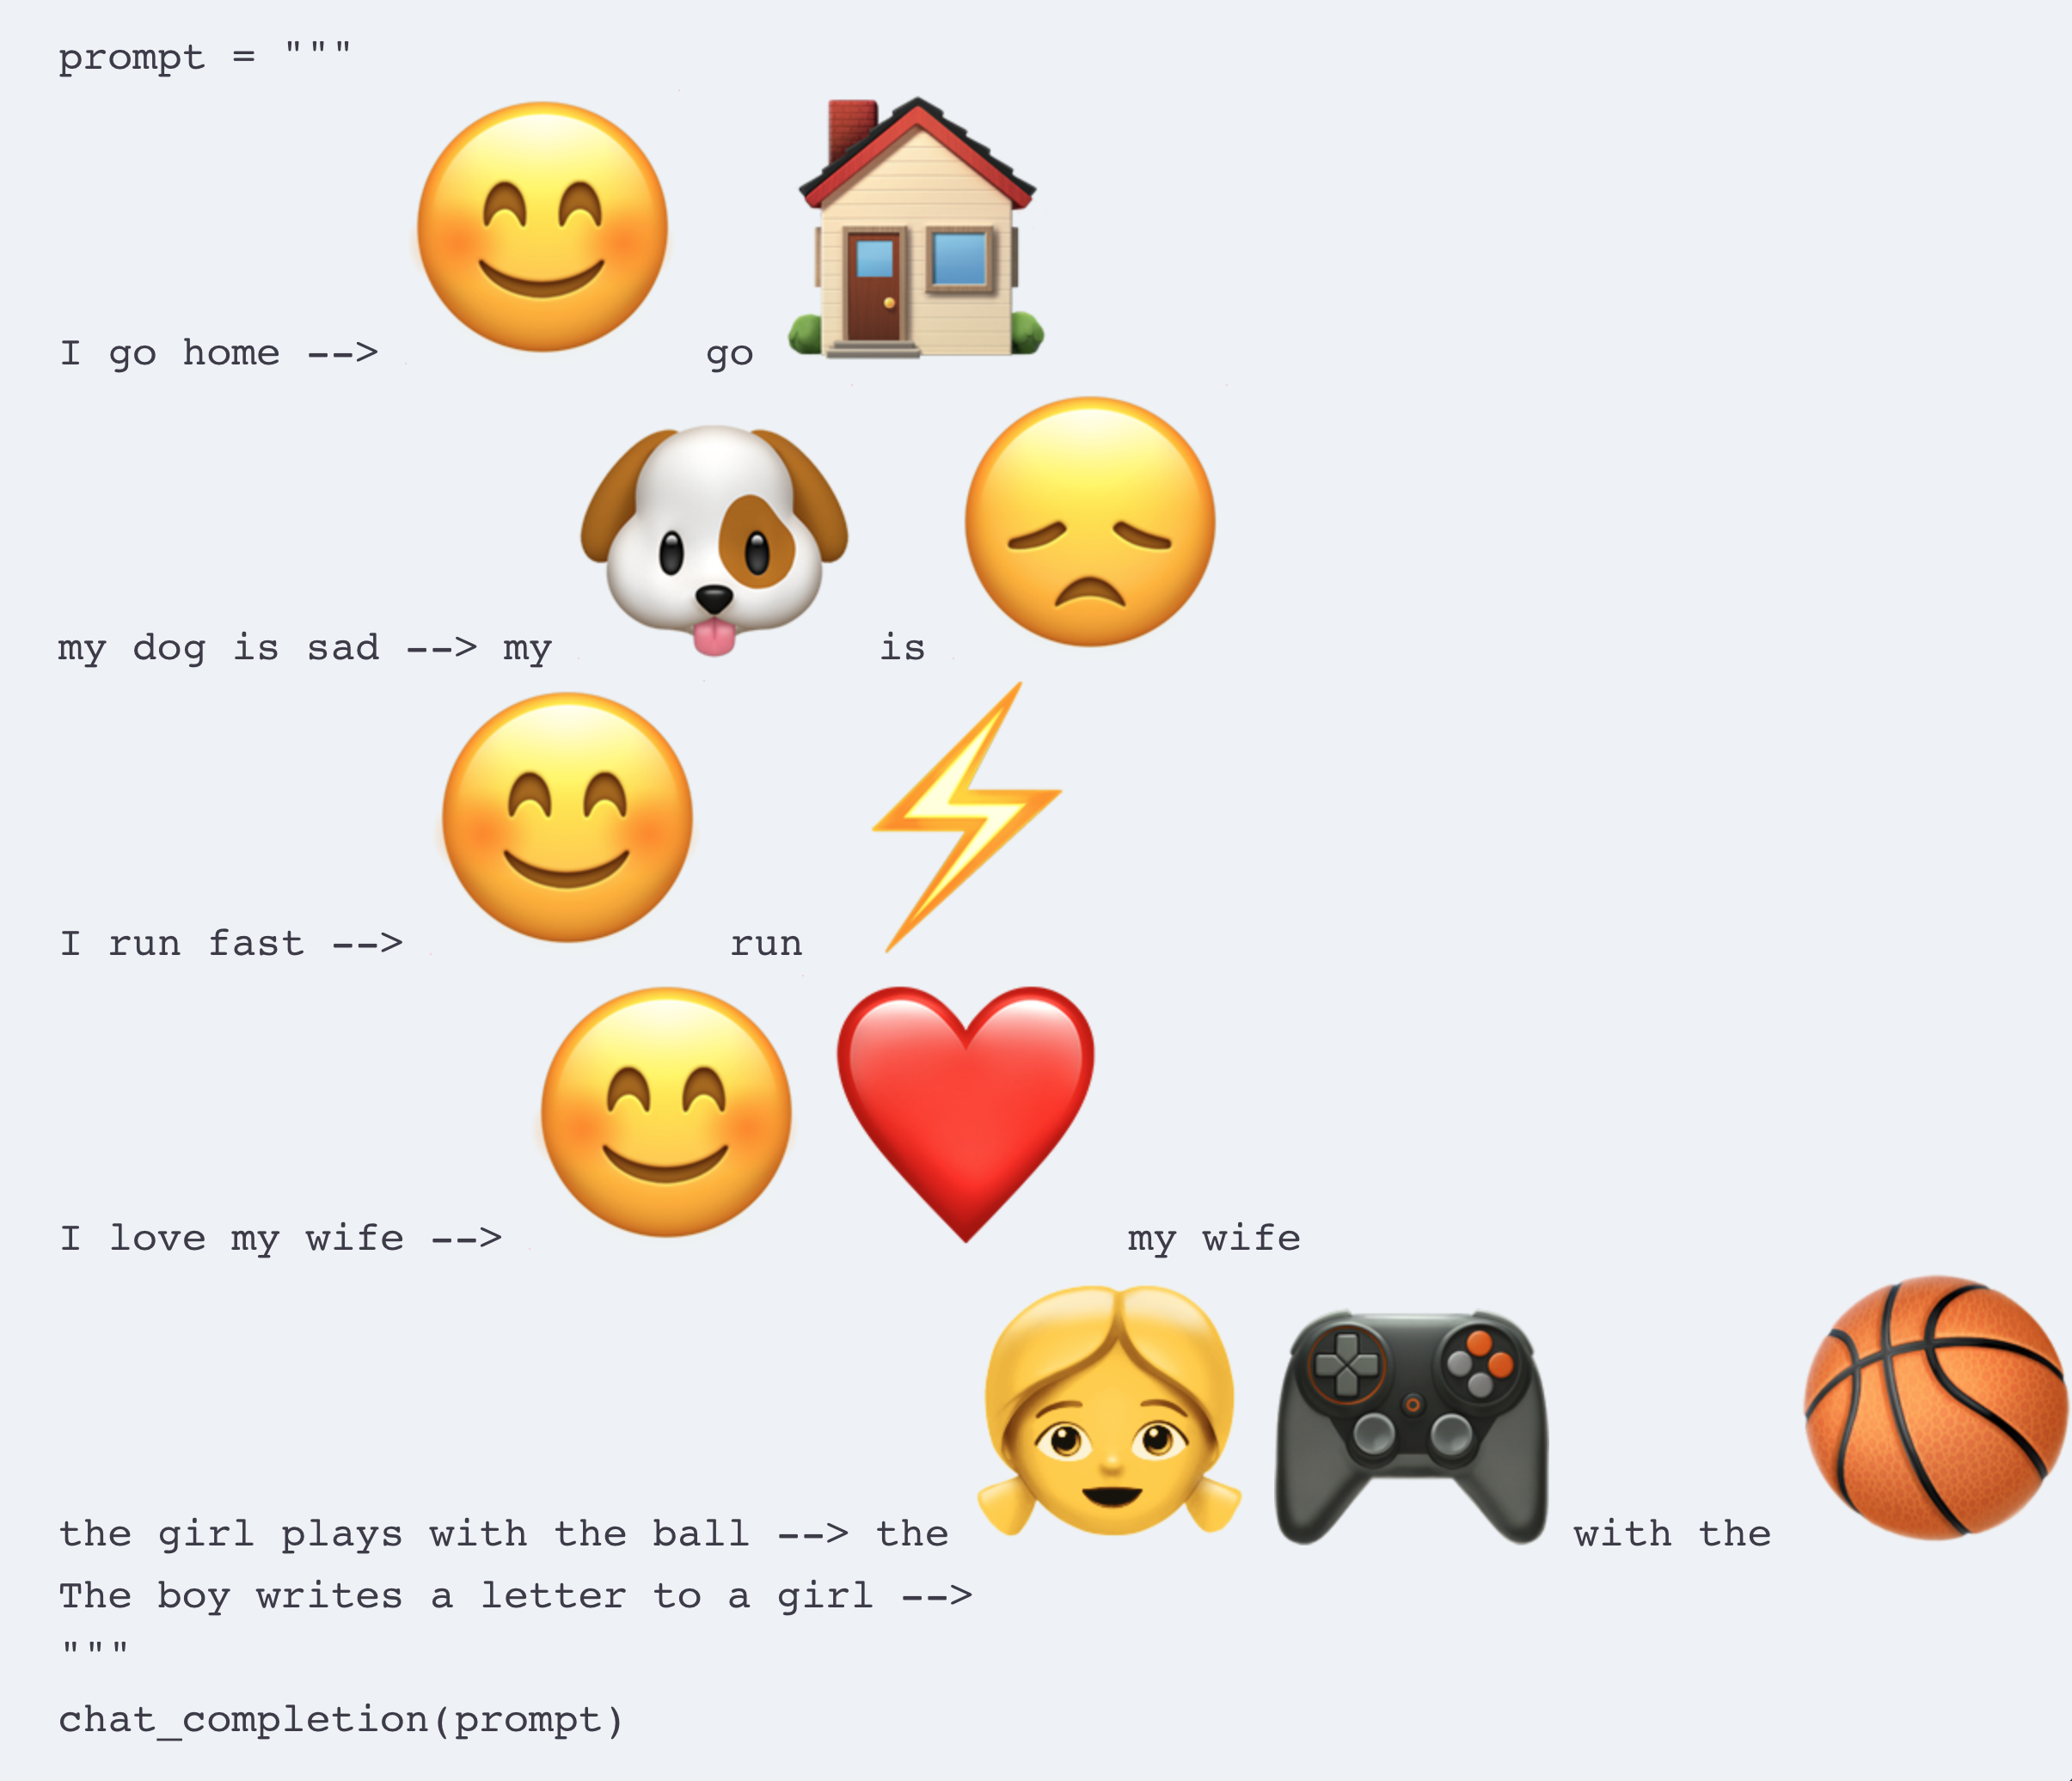
\includegraphics[width=0.8\textwidth]{figures/prompt-few-shots-question.png}
\objectsource{\textcite{Olivier2024}}
\end{figure}
% End Figure ---------------------------

Moreover, we get as output the following message:

% Start Figure ----------------------------
\begin{figure}[ht]
\caption{A prompt few-shot answers}
\centering
\label{fig-prompt-few-shots-answers}

\includegraphics[width=0.8\textwidth]{figures/prompt-few-shots-answer.png}
\objectsource{\textcite{Olivier2024}}
\end{figure}
% End Figure ---------------------------

The few-shot learning technique provides examples of prompts with the desired outcome. The final line contains the prompt for which a completion is desired, in the same form as the above examples. The language model will then perform a completion operation, considering the pattern of the examples above.

One can be amazed at how effortlessly the model grasps and reproduces instructions with just a handful of examples. This is achievable due to the vast knowledge LLMs accumulate during their training, enabling them to adapt and furnish precise responses based on minimal examples. The capacity to learn from a few examples is a potent attribute of LLMs, making them incredibly versatile and flexible while only needing a small amount of supplementary information to accomplish diverse tasks.

When providing examples in the prompt, it is essential to ensure the context is clear and relevant. Clear examples help the model better understand the desired output format and the problem-solving process. Conversely, inadequate or ambiguous examples can lead to unexpected or incorrect results. Therefore, writing examples carefully and ensuring they convey the correct information can significantly impact the model's ability to perform the task accurately.

Another approach to guiding LLMs is one-shot learning, which involves providing only one example to help the model understand the task. This approach is simpler, faster, and less computationally intensive than few-shot learning. One-shot learning can be effective for straightforward tasks or when the LLM already has significant background knowledge about the topic. However, for more complex tasks or situations that require a deeper understanding of the desired outcome, few-shot learning may be a better approach to ensure accurate results.
To optimize the performance of LLMs, we have explored various techniques of prompt engineering. This process involves refining the prompt to guide the model more effectively, which can lead to better results, especially when dealing with more complex tasks. 

\subsection{AI tools for developers}
Building on the same technology as LLMs like GPT-3~\cite{Brown2020}, AI-powered code completion tools such as GitHub Copilot\footnote{\url{https://github.com/features/copilot}} (built on OpenAI’s Codex model ~\cite{MarkChen2021}, Amazon’s CodeWhisperer\footnote{\url{https://aws.amazon.com/codewhisperer}}, and DeepMind’s AlphaCode\footnote{\url{https://alphacode.deepmind.com/}}, recommend code completions within an integrated development environment (IDE) to help programmers author software. These tools are projected to profoundly impact the productivity and experience of professional programmers and, more broadly, anyone engaging in programming tasks~\cite{Ziegler2022productivity}.

GitHub Copilot, an "AI pair programmer," is optimized for code auto-completion. It completes a given initial code snippet, whether it's a method's documentation, signature, or partial implementation~\cite{MarkChen2021}. Based on the OpenAI Codex model\footnote{\url{https://platform.openai.com/docs/guides/code}}, a 12 billion parameter version of GPT-3~\cite{Brown2020}, Copilot has been fine-tuned using code samples from 54 million public software repositories on GitHub.

Beyond auto-completion, Copilot can explain code, generate documentation, and translate code between languages. However, its effectiveness can fluctuate, especially when a developer's intent is unclear. Developers often have a general idea but lack specifics such as suitable functions, libraries, or algorithms.

Studies have shown mixed results regarding Copilot's impact on productivity. Some discovered increased users' perceived productivity~\cite{Ziegler2022productivity} and acceptance of proposed code completions~\cite{Vaithilingam2022}. In contrast, others found no significant improvement in task completion times or success rates~\cite{Vaithilingam2022}. Interestingly, a study by~\cite{Ziegler2022productivity} showed that developers using Copilot implemented a JavaScript web server 55\% faster than those not using it.

An analysis of programmer interactions with Copilot showed that the effectiveness of autocompletion depends on whether developers were speeding up familiar tasks ("acceleration mode") or exploring unfamiliar problem solutions ("exploration mode"). Developers often iteratively type comments, review Copilot's responses and modify their comments to explore other potential solutions. These comments are usually deleted after the relevant code is generated, reflecting their temporary function in this iterative refinement process.

However, the imperfection of these models can lead to challenges. They often struggle to distinguish correct outputs from seemingly coherent and plausible ones, leading to potential bugs or security vulnerabilities. This has gained widespread attention since the release of ChatGPT.

For effective human-AI collaboration in coding, programmers must be able to detect and correct any errors introduced by the code completion tool, which can be a challenge due to potential automation bias, overreliance, and automation-induced complacency~\cite{Wickens2015}. Therefore, conveying AI uncertainty and providing explanations is crucial, particularly in high-stakes domains like medical~\cite{Lundberg2018}, legal~\cite{Pagliario2022}, and hiring. However, translating these strategies into generative scenarios with complex outputs, where operators face numerous small decisions, remains unclear.


\section{Software Patterns}\label{sec:software-patterns}
Patterns are not an exclusive aspect of Software Engineering. Psychologists identify patterns of behavior upon which they can take one action or another; Economists look for patterns in changes in stock prices that support their buying and selling policies. 

Software Patterns are solutions to recurring software problems. These solutions are the result of the experiences of experts and can be used over and over again~\cite{Gamma1994}. Software patterns can be categorized into classes according to the software development phase. Implementation patterns, testing patterns, analysis patterns, architectural patterns, and design patterns are examples of these classes~\cite{Hamza2004} and are an active field of research in software engineering~\cite{Zhang2011, Zhang2013, Riaz2015}.

\subsection{The Origin of Pattern Theory}\label{sec:origin-pattern}
The ideas behind \ac{DP}, as we know them today, are derived from the patterns for buildings and urban planning design presented by Christopher Alexander, who wrote the following definition of an architectural pattern: 
\textit{``Each pattern describes a problem which occurs over and over again in our environment, and then describes the core of the solution to that problem, in such a way that you can use this solution a million times over, without ever doing it the same way twice."}~\cite[p.~10]{Alexander1977}. 

Although not required, it is recommended to use patterns when solving problems. If a pattern already exists for a particular issue, you can use it or create a new one. It is important to remember that a pattern represents the foundation of a solution, as defined by Alexander. While it can be utilized, it should never be applied in the same way more than once.

Alexander’s idea was used by Kent Beck and Ward Cunningham in 1987 to facilitate the teaching of human-computer interfaces using object orientation, and a pattern comprises the following two essential areas: the recurring problem of the environment and the description of the resulting solution to be reused~\cite{Beck1987}. A good standard should meet the following characteristics~\cite{Coplien2004}:

\begin{itemize}
    \item \textbf{Solves a problem:} A pattern captures solutions, not just abstract principles or strategies.
    \item \textbf{It is a proven concept:} Patterns are industry-proven solutions, not theories or speculation.
    \item \textbf{The solution is not obvious:} Many problem-solving techniques seek solutions from basic principles. The best patterns indirectly generate a solution to a problem, a necessary approach to the most challenging design problems.
    \item \textbf{Describes a relationship:} Patterns describe the system's modules and deeper structures and mechanisms.
    \item \textbf{The standard has a significant human component:} All software serves the comfort or quality of human life. Better standards make the software easier for people to use and maintain. 
\end{itemize}


\subsection{Design Patterns of Gang of Four}\label{sec:gof}
The success of \ac{DP} had to wait until 1994 when the Gang of Four(GoF) published the book Design Patterns: Elements of Reusable object-oriented software~\cite{Gamma1994}. This book contains twenty-three design patterns from the author's extensive personal experience.
 
\ac{DP} have been organized into three categories, each defining different problems. They are categorized into creational, structural, and behavioral patterns, described in Board~\ref{board:pattern-category} above:

\begin{table}[ht]
    \centering
     \footnotesize
     \setlength{\tabcolsep}{4pt}
    \caption{The Design Patterns organized by category}
    \label{board:pattern-category}
    \begin{tabular}{lp{.59\linewidth}rp{.01\linewidth}cp{.01\linewidth}} 
        \toprule
         \hline
        \rowcolor{gray!19} \textbf{Category} & \textbf{Patterns Name} & \textbf{Amount} \\
        \hline
        Creational & Abstract Factory, Builder, Factory Method, Prototype, Singleton & 5 \\
        \rowcolor{gray!19} Structural & Adapter, Bridge, Composite, Decorator, Facade, Flyweight, Proxy & 7 \\
        Behavioral & Chain of Responsibility, Command, Interpreter, Iterator, Mediator, Memento, Observer, State, Strategy, Template Method, Visitor & 11 \\ 
        \hline
        \bottomrule
    \end{tabular}
    \objectsource{\objectsourceauthor}
\end{table}

\begin{itemize}
\item \textbf{Creational:} They are standard ways of dynamically creating new objects at the execution time of a program. Their main goal is to make the code that is being used by some objects independent of the classes that define these objects, according to the open-closed design principle for proper object-oriented design;

\item \textbf{Structural:} They are related to standard ways of dynamically creating objects that reuse existing class hierarchies;

\item \textbf{Behavioral:} This category division the responsibilities into different classes and defines the communication between their objects at the execution time of a program.
\end{itemize}

\subsection{Design Pattern Selection Methods} \label{sec:pattern:selection-methods}
Software design patterns have a considerable impact on the software development life cycle. However, due to the many design patterns, selecting the appropriate one is quite difficult. Several approaches with different methods have been presented to overcome this difficulty to indicate the appropriate \ac{DP}. The following subsections summarize the literature review on design pattern selection methods.

\MyPara{UML-Based Approach}\label{subsec:uml-approach}

The UML-based approach provides a set of "visual" descriptive graphical and textual techniques that system developers easily understand was selected some existing studies for selecting a design pattern based on the UML approach. The process of suggesting patterns in this approach is shown in Figure \ref{fig-uml-based-approach}. The first step in the process is a formal specification of the problem/solution domain using UML diagrams as a meta-model. The UML includes several class, collaboration, and sequence diagrams used to describe the meta-model. The next step is to specify different aspects of the patterns to obtain different properties, such as structural and behavioral. Finally, mapping is performed, and if the design pattern specifications can satisfy the problem diagram, a design pattern is suggested~\textcite {Hsueh2009} and~\textcite{Kim2007, Kim2008} used this approach to suggest suitable design patterns.

% Inicio Figura ---------------------------
\begin{figure}[ht]
\caption{Overview of UML-Based Approach.}
\centering
\label{fig-uml-based-approach}
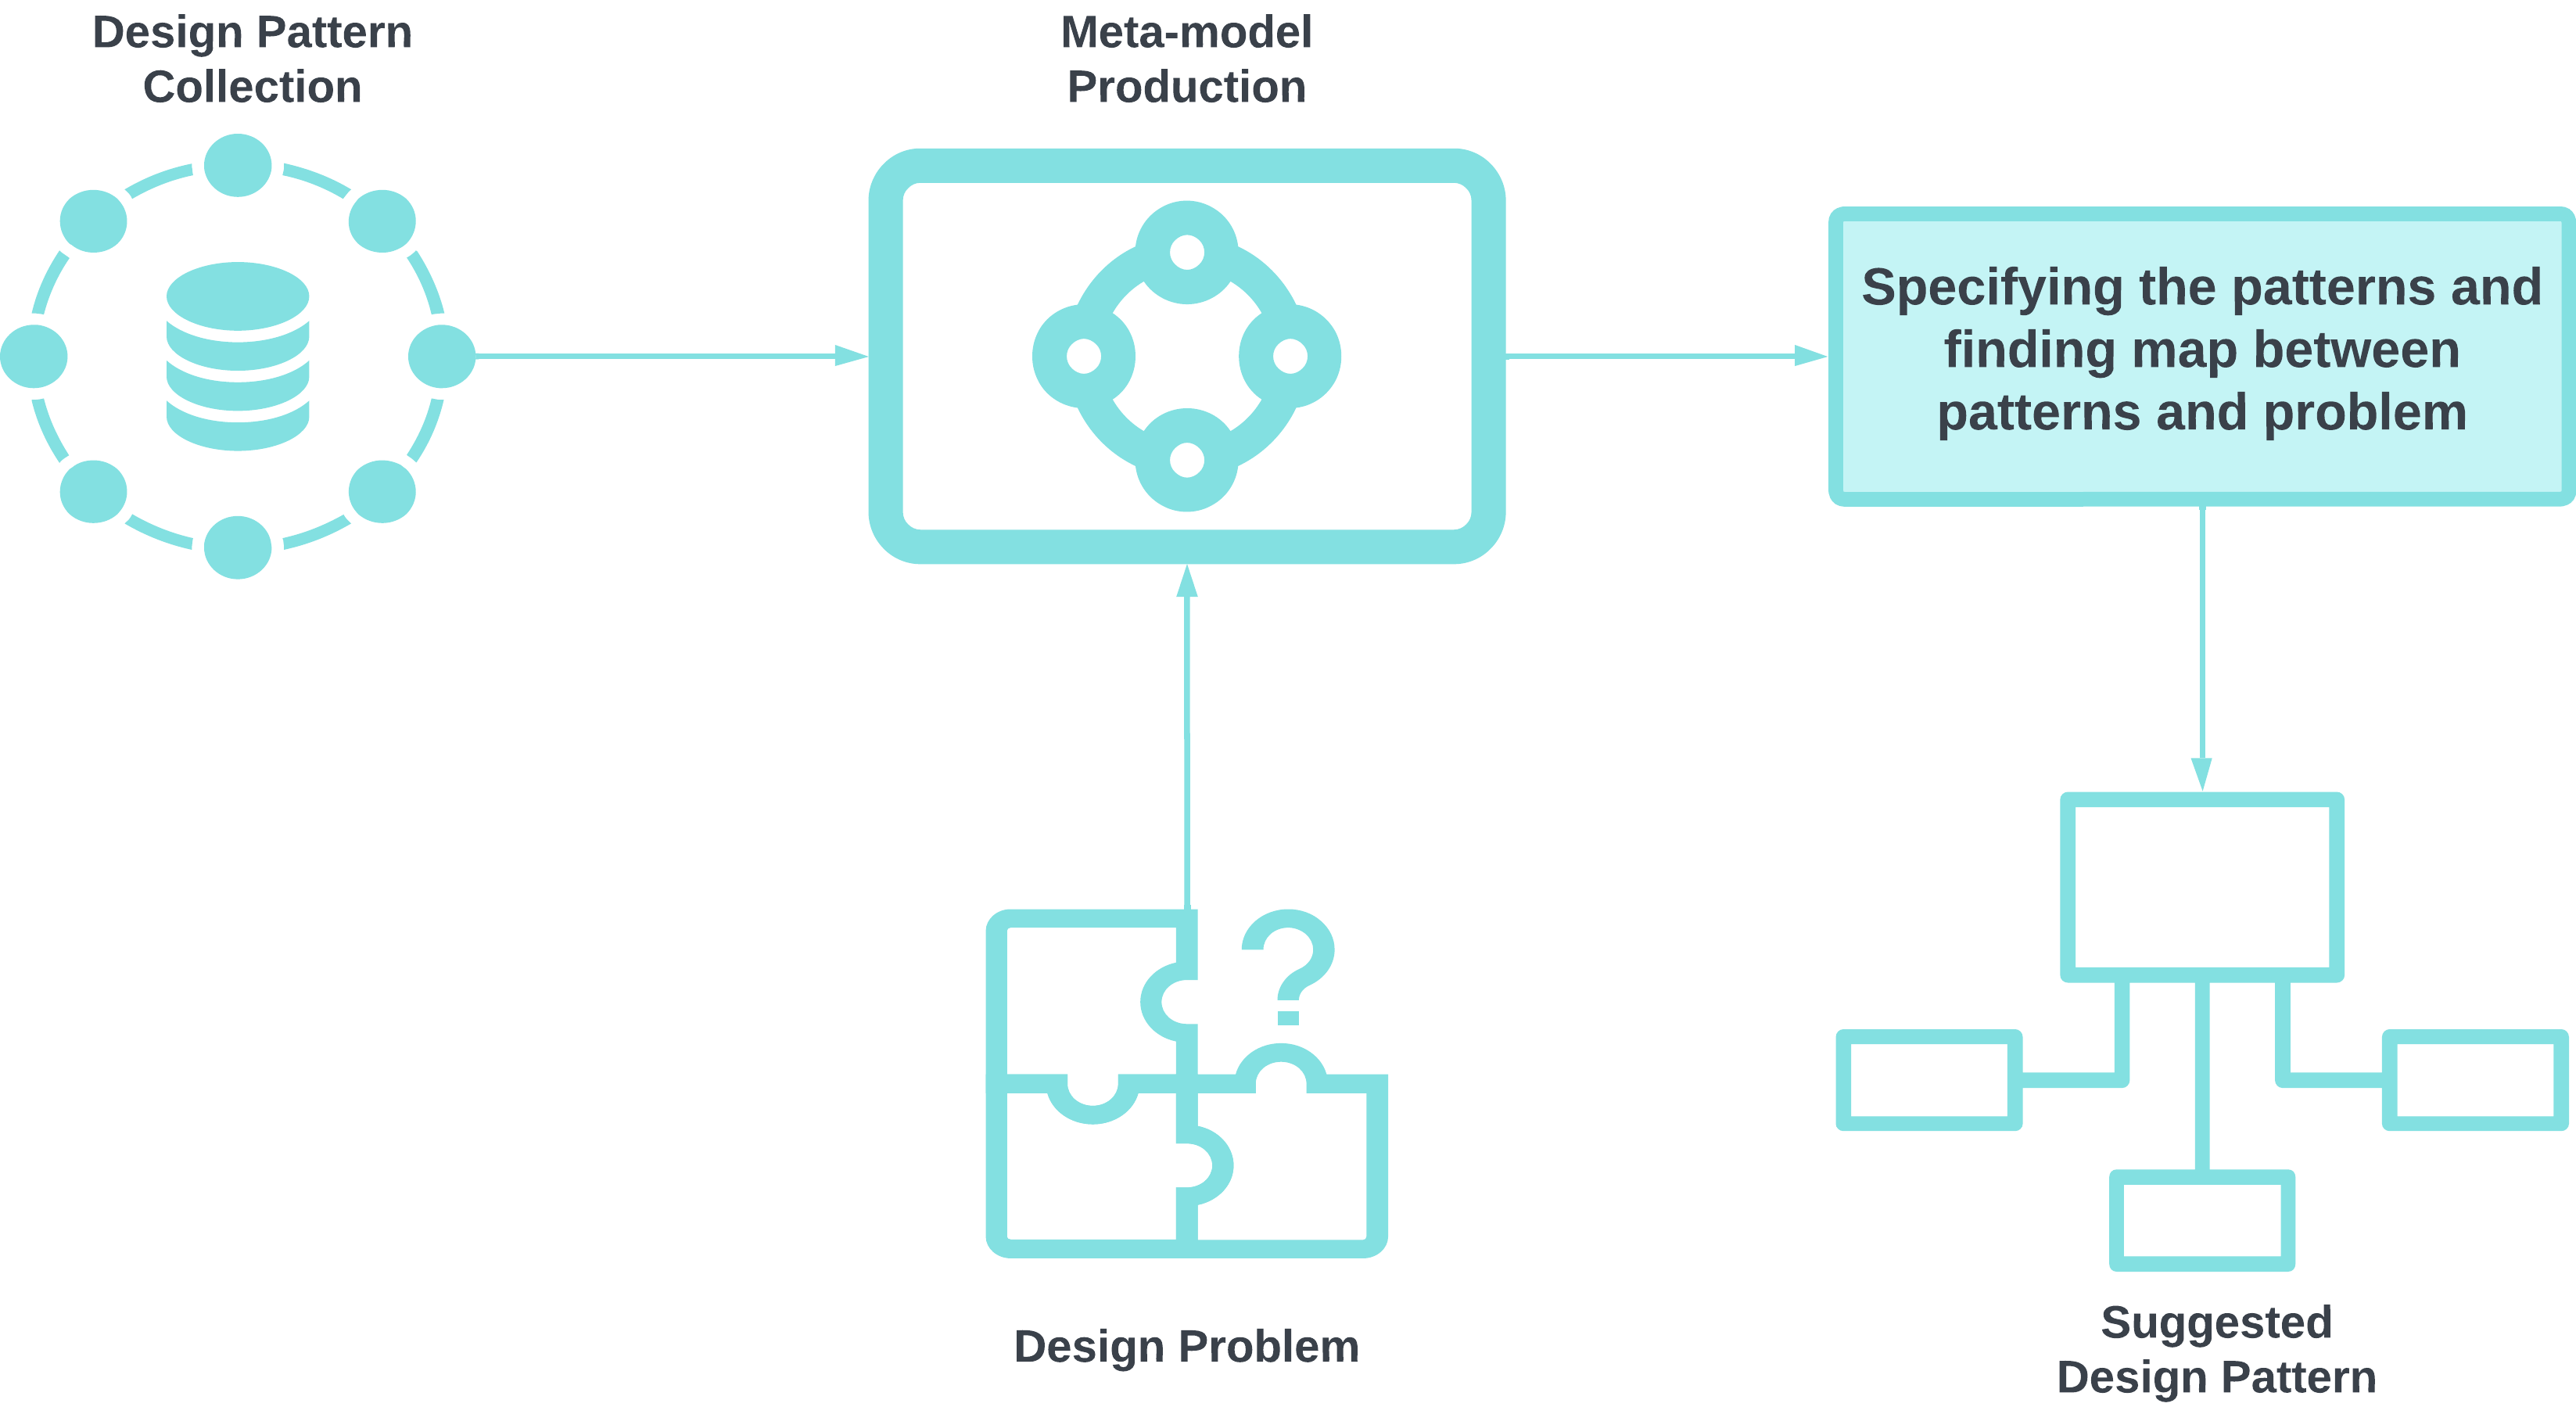
\includegraphics[width=0.9\textwidth]{figures/uml-based-selecion-pattern-approach.png}
\objectsource{\objectsourceauthor}
\end{figure}
% Fim Figura ---------------------------

However, this approach has two limitations. Firstly, some patterns have similar structures but different intentions, such as State, Strategy, Façade, and Adapter patterns, resulting in similar meta-models. Secondly, due to the overhead of generating meta-models, the scalability of this approach is limited. As the number of patterns augments, the similarity between meta-models also increases.

\MyPara{Question-Answer-Based Approach}\label{subsec:question-answer-approach}

The question-answer-based approach involves developers presenting multiple questions and suggesting appropriate patterns based on the user's responses. Figure~\ref{fig-question-answers-base-approach} demonstrates the process for suggesting patterns using this approach, which involves creating intermediate representations like trees and rules from the design pattern description and suggesting patterns based on user interaction.

% Inicio Figura ---------------------------
\begin{figure}[ht]
\caption{Overview of question-answer based approach.}
\centering
\label{fig-question-answers-base-approach}
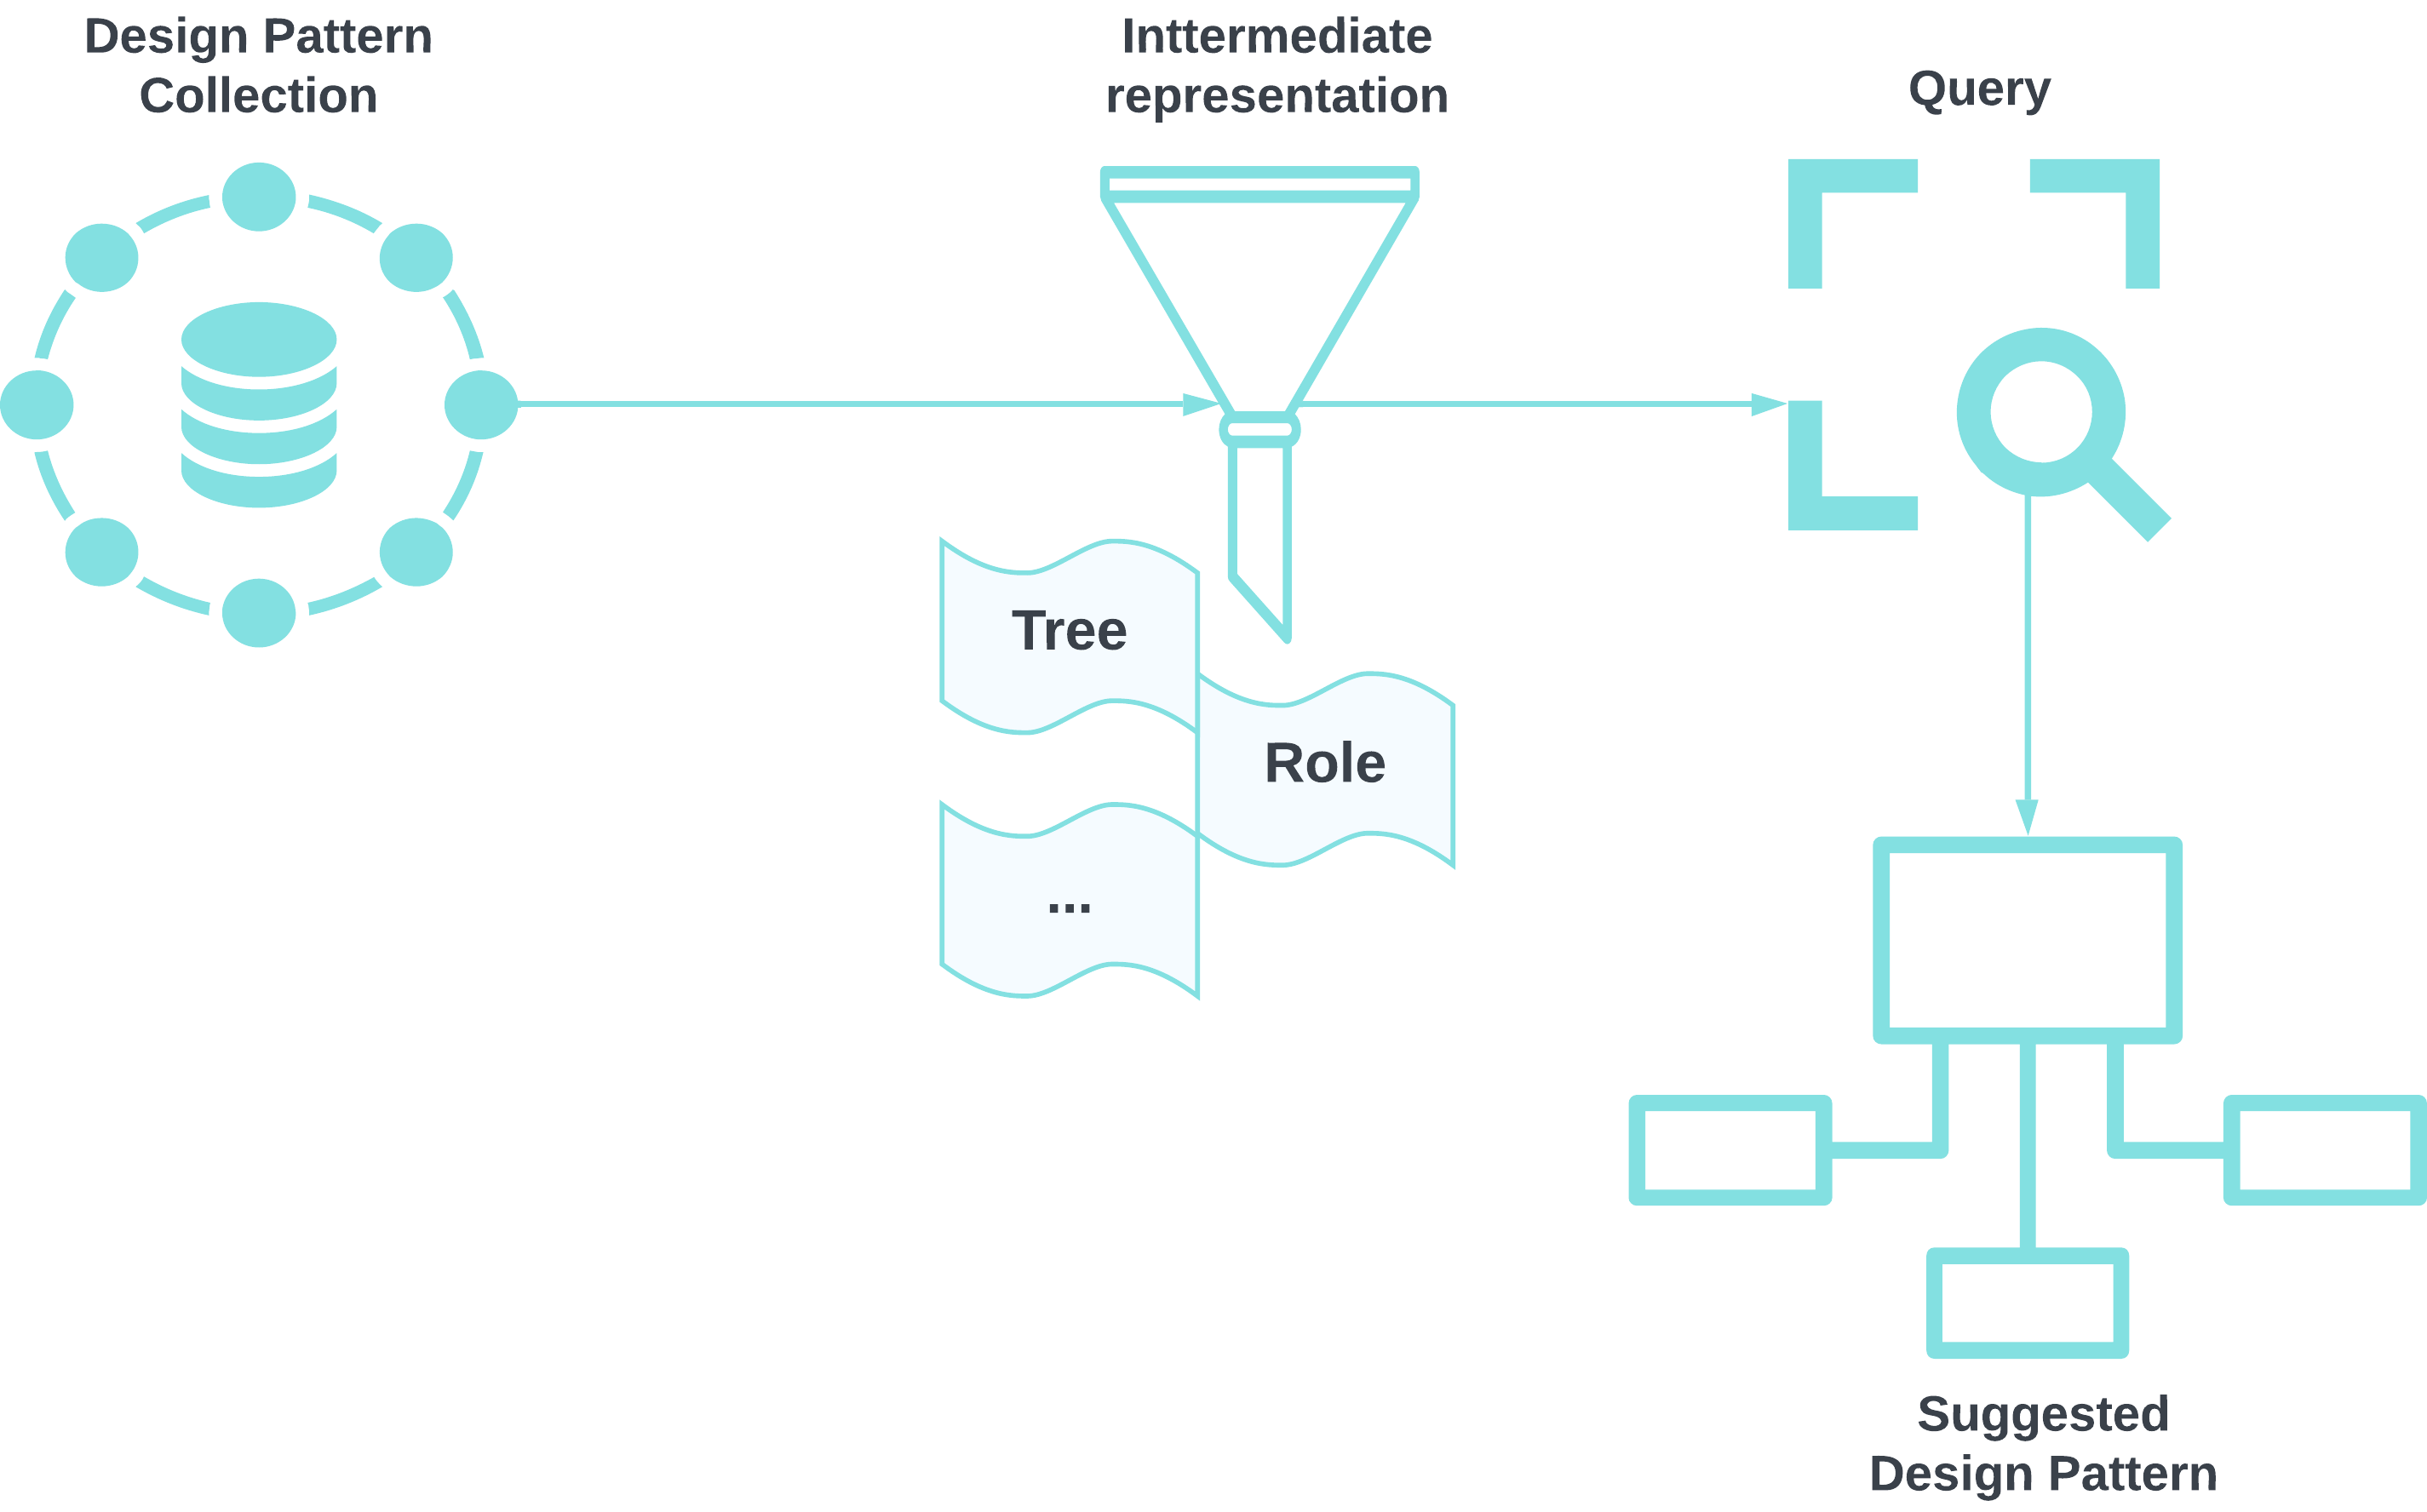
\includegraphics[width=0.9\textwidth]{figures/question-answers-select-pattern-approach.png}
\objectsource{\objectsourceauthor}
\end{figure}
% Fim Figura ---------------------------

Many researchers, including~\textcite{Gueheneuc2007},~\textcite{Palma2012},~\textcite{Pavlivc2014},~\textcite{Sanyawong2014},~\textcite{Navarro2010},~\textcite{Issaoui2015},~\textcite{Diaz2010, Diaz2011} have utilized this approach to suggest appropriate design patterns.

The work of~\textcite{Palma2012} proposed a \ac{GQM} model for pattern selection. This model provides the conditions and sub-conditions of the design pattern, which are questions from the intent and applicability parts of the pattern description. A hierarchical tree is then presented, with each node containing a question. After the user interacts with the system and provides responses, the responses are weighted, and the design pattern with the highest weight (similarity) is suggested to the designer.

The model evaluation has been done by a total of six graduate students, along with two information technology professionals. The evaluation outcome resulted in a success ratio of 50\%. While~\textcite{Pavlivc2014} used the question-answers to build an ontology-based model for design pattern recommendations.

Nevertheless, constructing the questions in this approach is challenging, especially with many patterns. Furthermore, the questions are usually biased toward the specifics of the design patterns rather than the software design problem.

\MyPara{CBR-Based Approach}\label{subsec:cbr-approach}

The \ac{CBR} Based Approach uses old experiences to understand and solve new problems. Each of the experiences stored in memory is called a case. Each case in \ac{CBR} represents a situation that can take different formats based on experience. Typically, each case consists of three parts; the problem, the solution, and the explanation that states how the solution solves the problem~\cite{Kolodner1992}. The process of pattern suggestion in this approach is shown in Figure~\ref{fig-cbr-approach}. A case base can have different formats, such as text, diagram, and ontology.

% Inicio Figura ---------------------------
\begin{figure}[ht]
\caption{Overview of CBR-Based approach.}
\centering
\label{fig-cbr-approach}
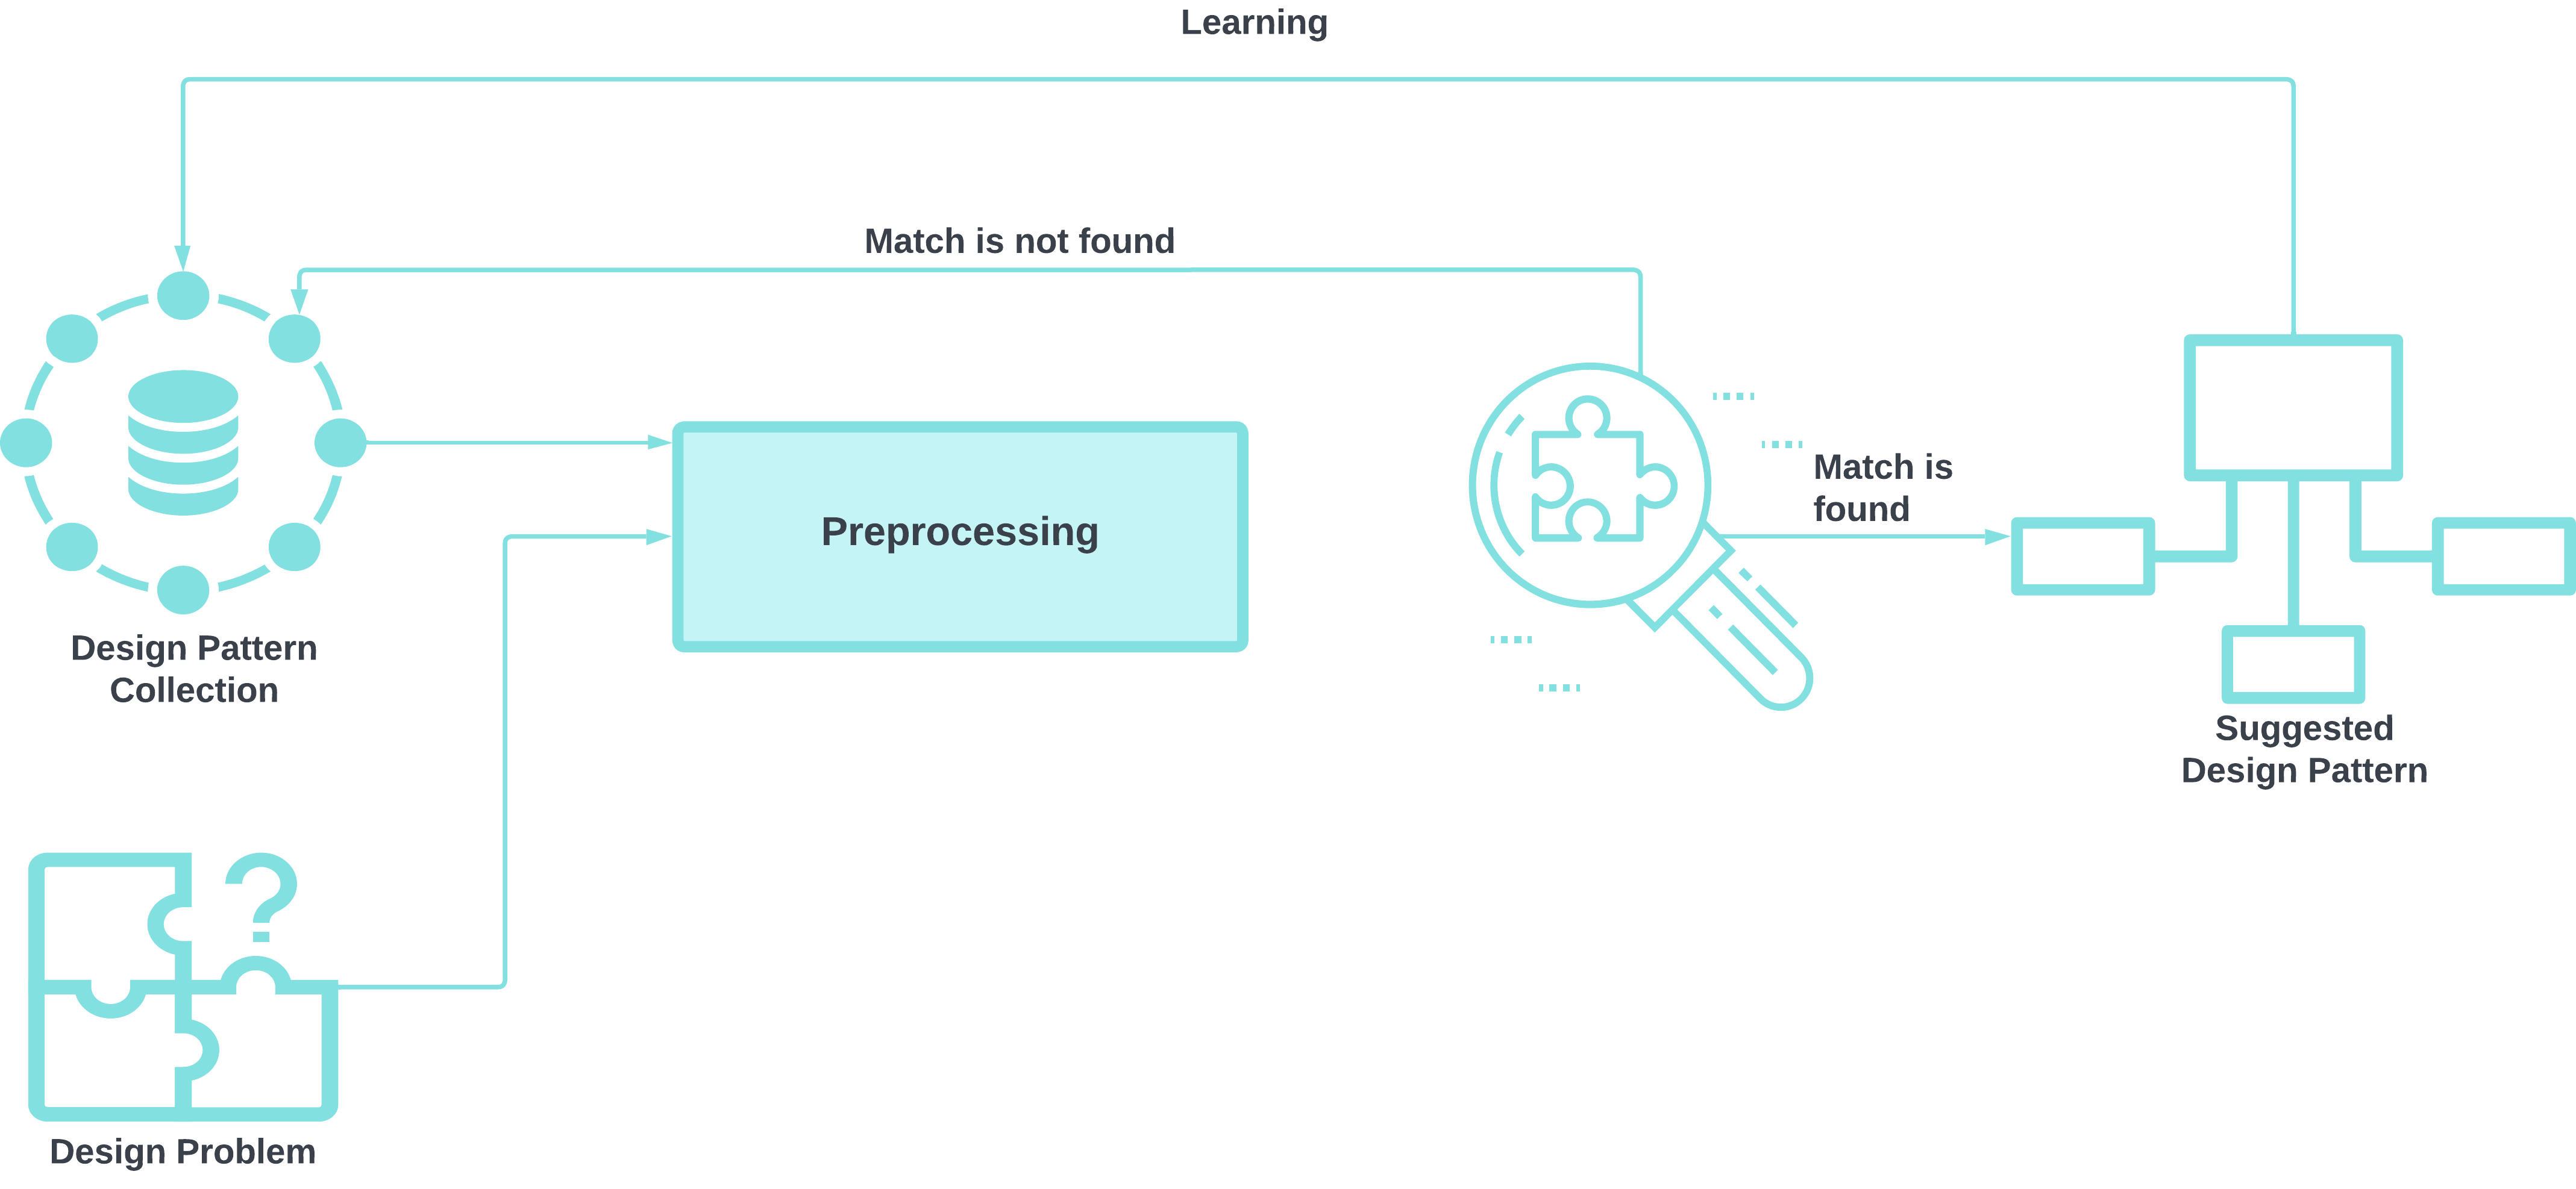
\includegraphics[width=1.0\textwidth]{figures/cbr-selection-pattern-approach.png}
\objectsource{\objectsourceauthor}
\end{figure}
% Fim Figura ---------------------------


In the first step, pre-processing is performed on the new case and the case base to achieve the desired representation for the applied method. In the second step, matching is performed to find the similarity between the new problem and the problems of the previous cases. In this step, if they can find a match, a new case from the problem and its solution will be created and added to the case repository in the learning phase. Otherwise, if they cannot find a match, adaption will occur, and the reason for failure is identified and added to the case base to prevent re-failure in subsequent problems. 

As a result, the \ac{CBR} system is enriched and improved by adding new cases to the case base~\cite{Avramenko2004}. ~\textcite{Muangon2013} has used this approach to suggest suitable design patterns.~\textcite{Gomes2002} presented a REBUILDER tool that provides new functionalities based on \ac{CBR}. The proposed method saves cases in a case base and is indexed using WordNet. Its knowledge base is constructed using examples of problem-specific cases to which design patterns are applied. 

Each case is a Design Pattern Application (DPA) in the form of UML diagrams that describe the specific situation in which the design pattern applies. A pattern is recommended based on a score obtained by mapping a domain-specific class diagram imported by a user with cases in the knowledge base.

\MyPara{Anti-Patterns-Based Approach}\label{subsec:anti-pattern-approach}

Design patterns offer practical solutions using tested formulas and methods to enhance development. However, anti-patterns provide reusable solutions that may seem helpful initially but eventually result in more harm than benefit. This can occur for various reasons, such as implementing the pattern in the wrong place or time~\cite{Nahar2016}. Every design pattern has several corresponding anti-patterns~\cite{Nahar2016improved}. Identifying these anti-patterns makes it possible to determine which patterns are inappropriate for a given problem.

Figure~\ref{fig-anti-pattern-approach} illustrates the pattern suggestion process in this approach. In the first phase, existing studies are examined to select a design pattern based on the corresponding anti-pattern approach. These studies are analyzed to identify the structural, behavioral, and semantic properties.

% Inicio Figura ---------------------------
\begin{figure}[ht]
\caption{Overview of anti-pattern based approach.}
\centering
\label{fig-anti-pattern-approach}
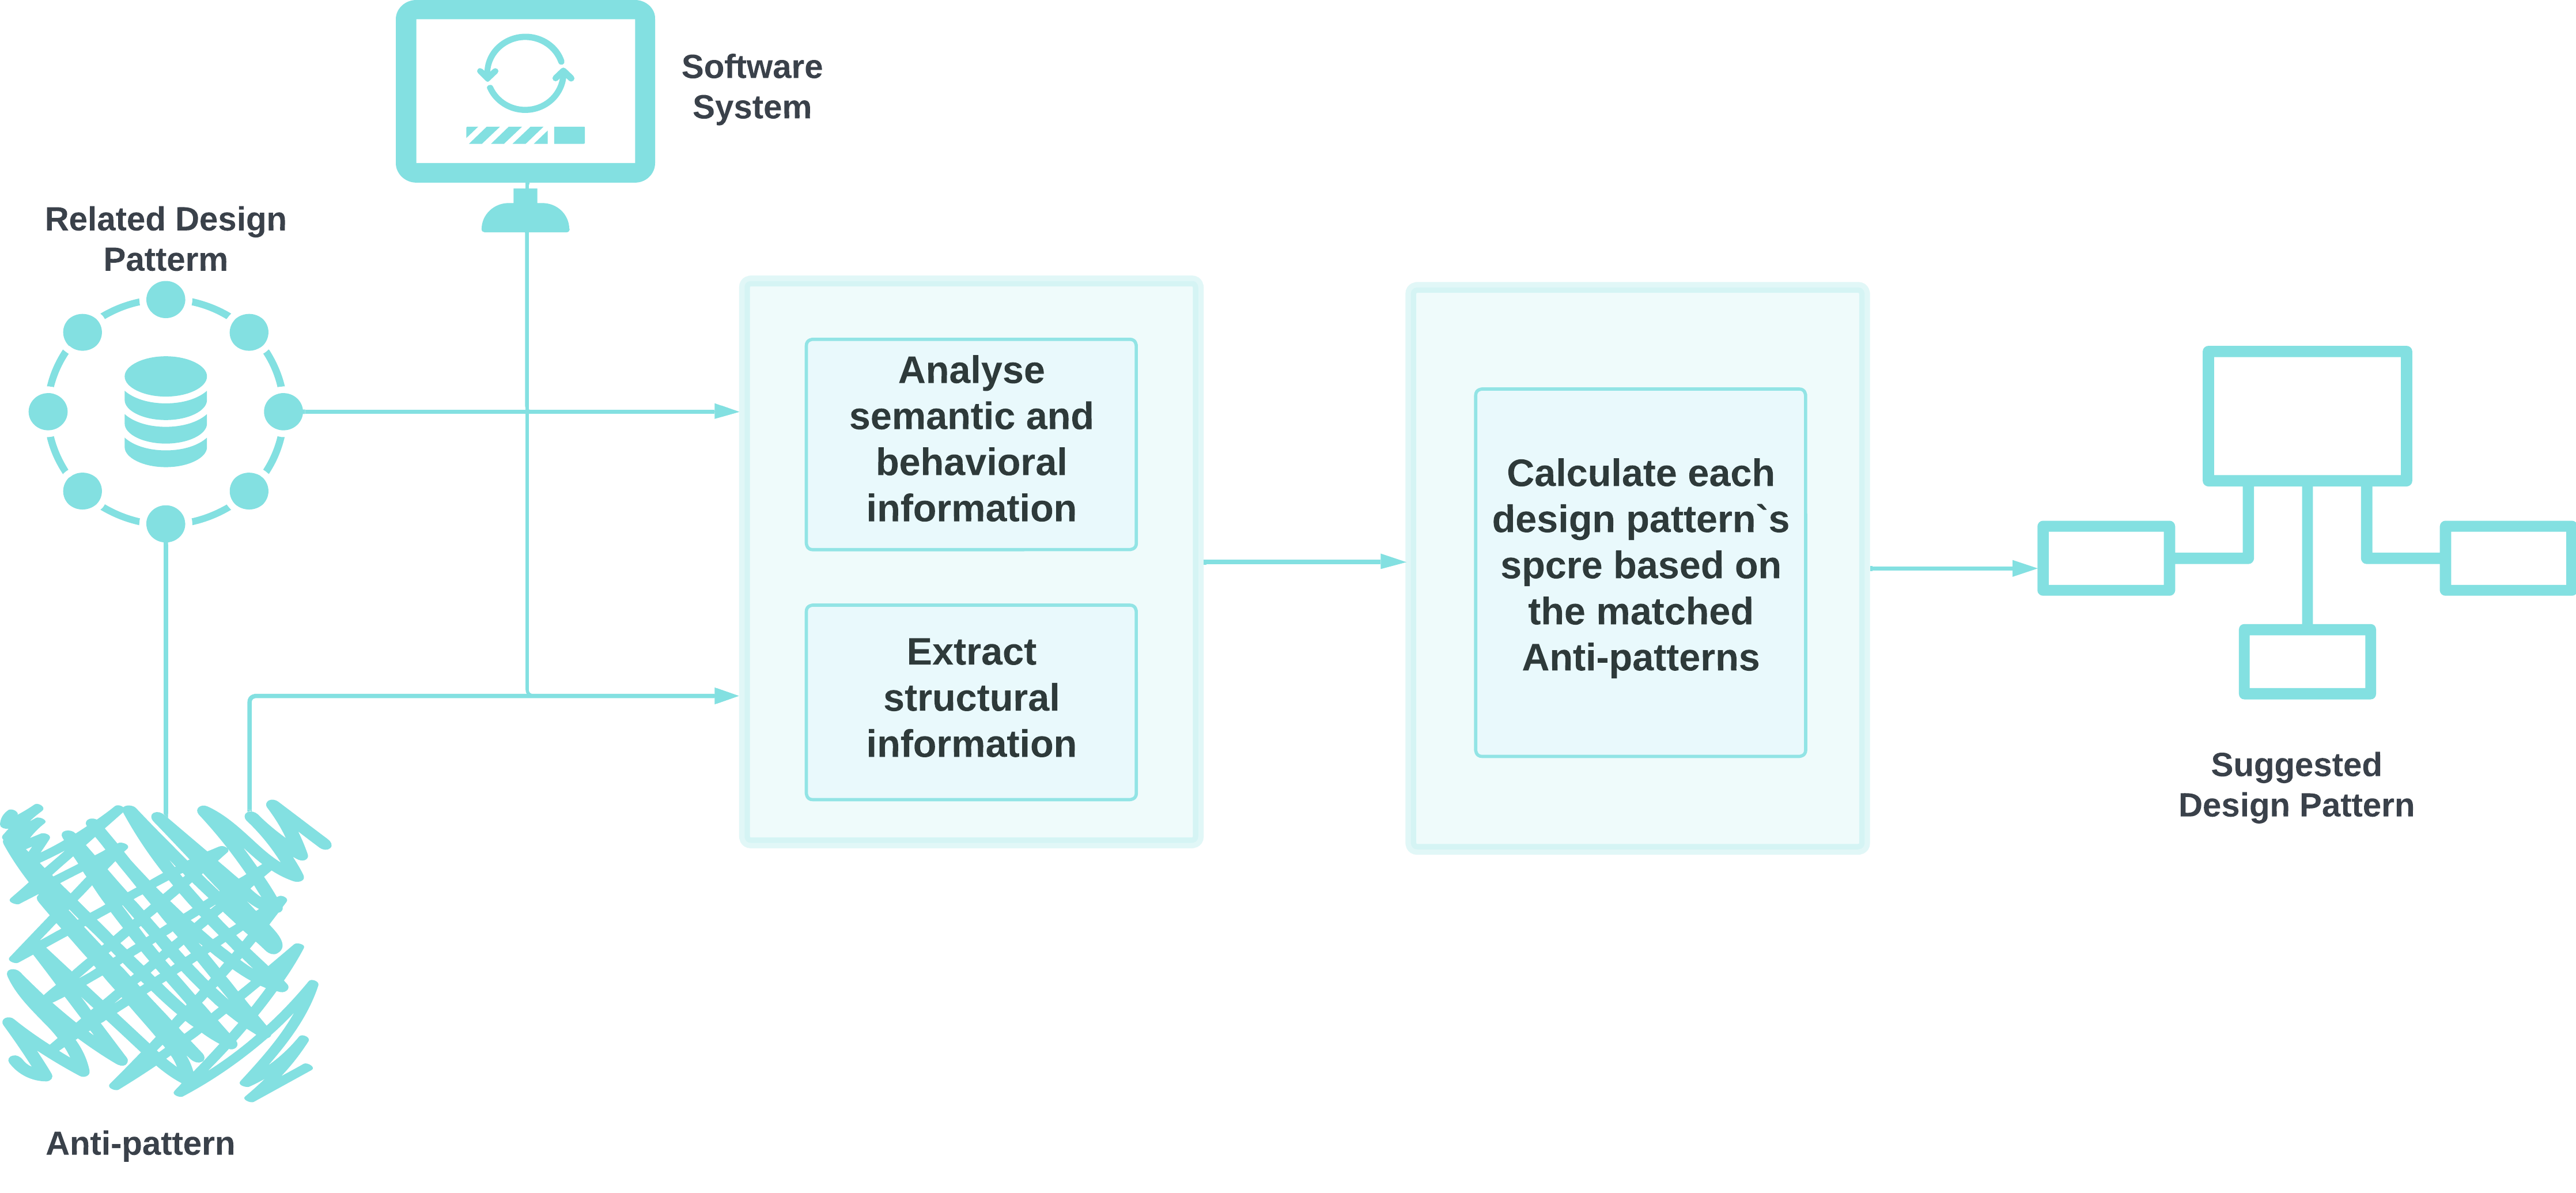
\includegraphics[width=1.0\textwidth]{figures/ant-pattern-selection-approach.png}
\objectsource{\objectsourceauthor}
\end{figure}
% Fim Figura ---------------------------

These three levels of analysis are performed to ensure the accurate capture of anti-pattern information. In the second phase, each design pattern obtains a score based on the match or mismatch of the structure, behavior, and semantics. If a design pattern gets the highest score, it perfectly fits that software design and is recommended ~\textcite{Bouhours2015, Nahar2015, Nahar2016, Nahar2016improved} have used this approach to suggest suitable design patterns.

~\textcite{Nahar2016} identified Anti-patterns corresponding to the design patterns in the software design phase and performed three structural, behavioral, and semantic analysis levels. Design patterns were then suggested based on their scores and the matching threshold value. However, a logical description of these anti-patterns has yet to be created.~\textcite{Smith2012} presented the same method for the Singleton pattern in the coding phase, which was not the right time since the software had already been developed.

\MyPara{Text-Classification-Based Approach}\label{subsec:text-classification-approach}

In Design Pattern Selection, two categories of text classification approaches, supervised and unsupervised processing algorithms, automatically suggest design patterns. Machine learning techniques classify Texts into specific classes based on one or more characteristics. Thus, there is no need for interaction with the designer, and the Design Pattern Selection process is fully automatic. The methodology overview of selecting a design pattern based on the text classification approach and the pattern suggestion process within this approach is shown in Figure \ref{fig-text-classification-based-approach}.

% Inicio Figura ---------------------------
\begin{figure}[ht]
\caption{Overview of text-classification-based approach.}
\centering
\label{fig-text-classification-based-approach}
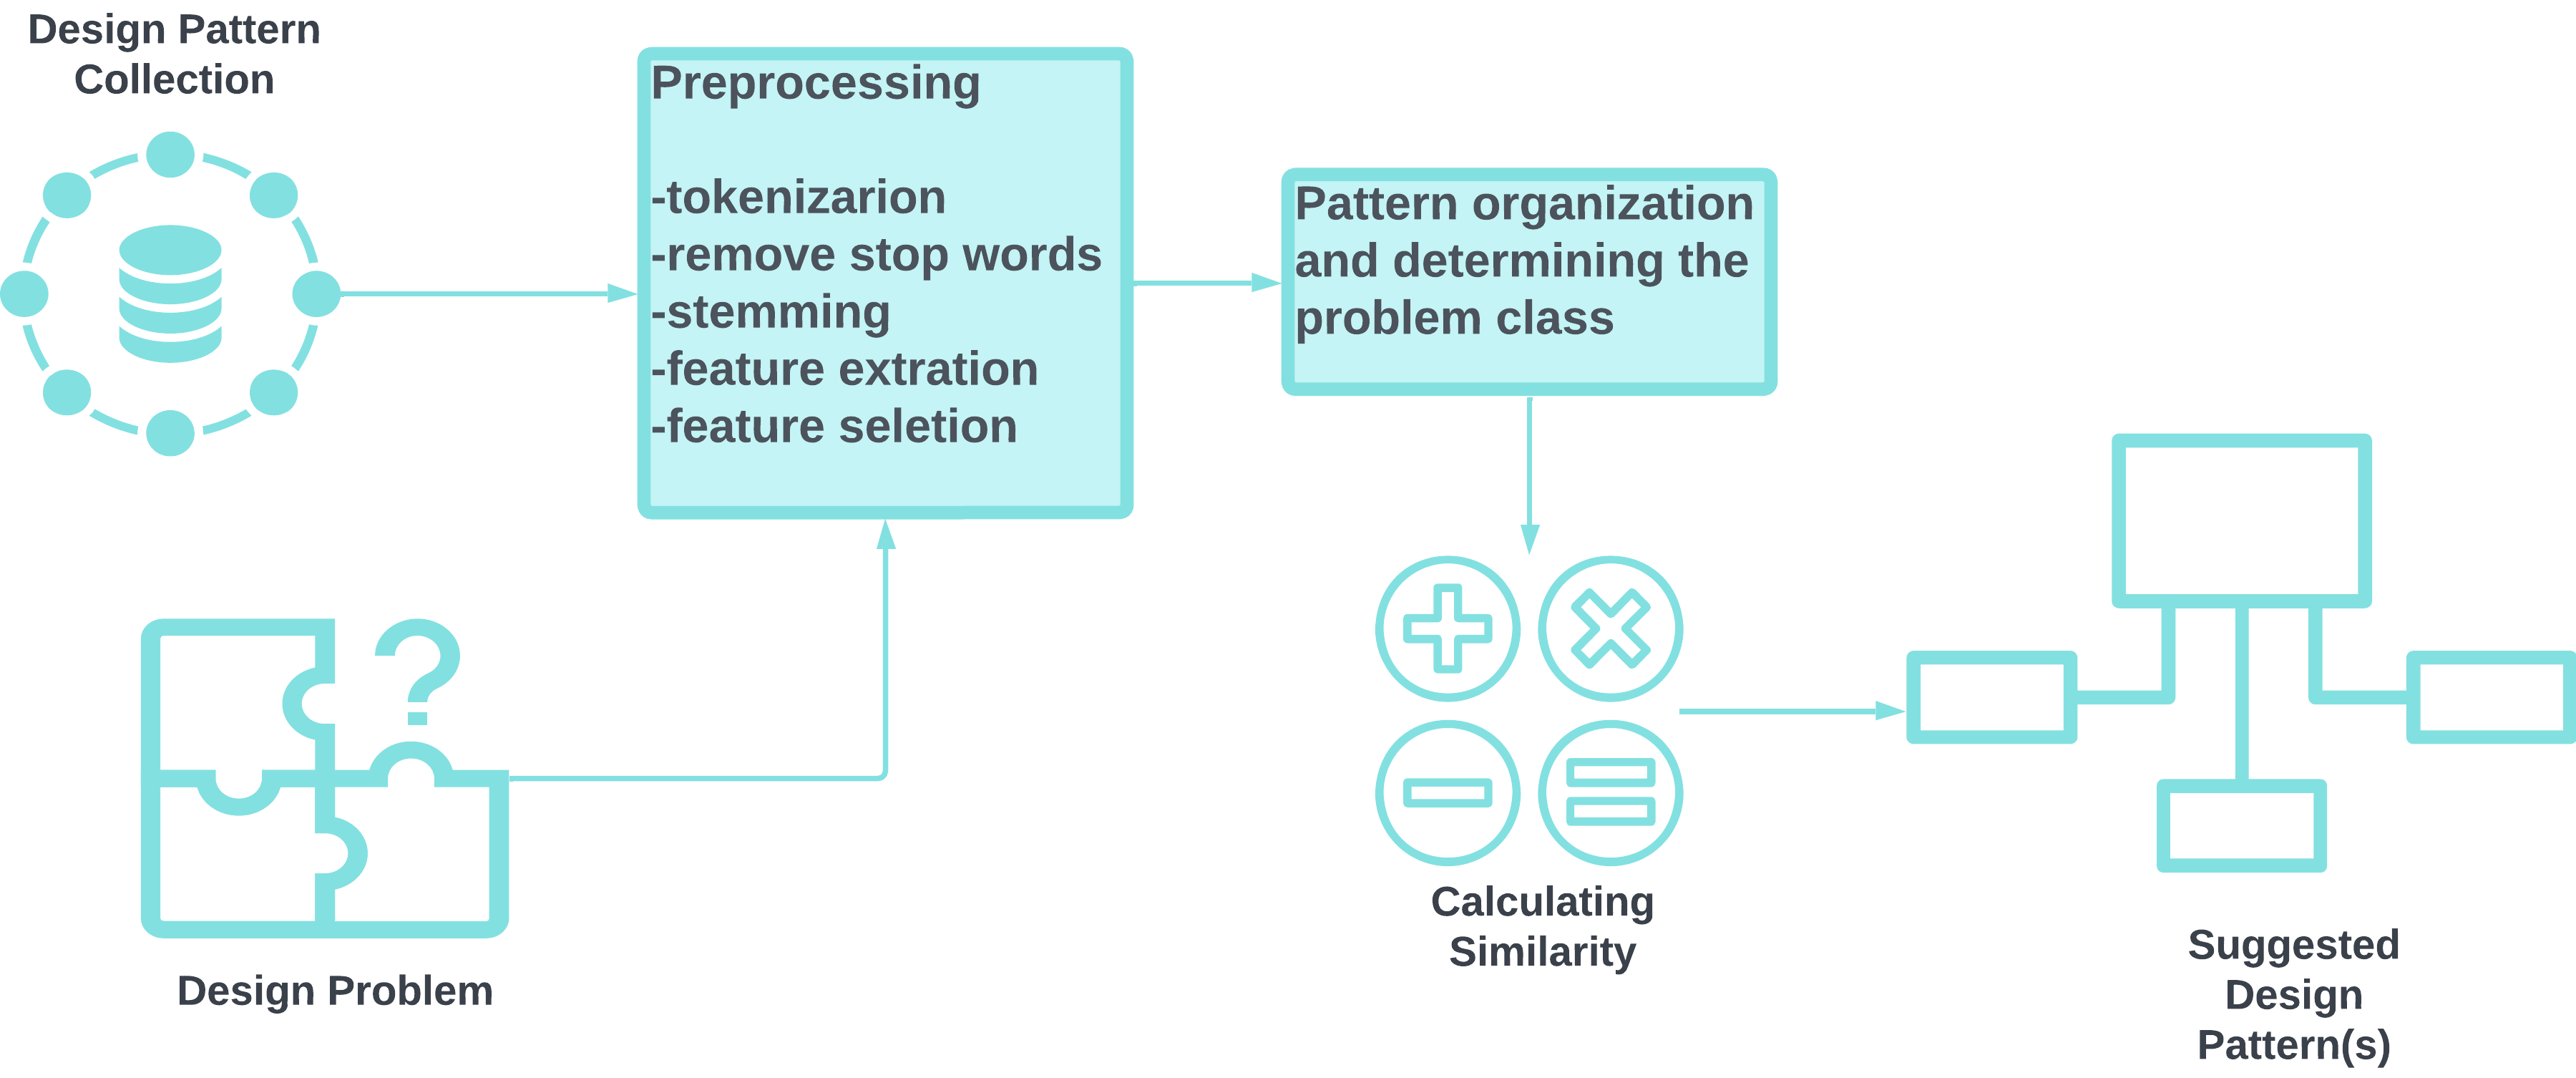
\includegraphics[width=1.0\textwidth]{figures/text-classification-selecion-pattern-aproach.png}
\objectsource{\objectsourceauthor}
\end{figure}
% Fim Figura ---------------------------

The prevalent types of machine learning are supervised, unsupervised, and semi-supervised learning. Supervised learning aims to create a learning model that can predict the true labels of unseen data while all data in the training set is labeled. Unsupervised learning aims to derive regular patterns by arranging unseen (unlabeled) data. Although the performance of the supervised learning method is excellent, the samples only sometimes contain the label information due to the high cost of labeling samples in the real world. 

On the other hand, unsupervised models almost underperform supervised models due to the need to find regular patterns ~\cite{Li2017}. Thus, in practical applications, the semi-supervised method, a composite of supervised and unsupervised learning, alleviates the need for supervision to a minimum. As this method explores a small number of labeled and many unlabeled samples, researchers in various fields have been using semi-supervised algorithms as an alternative to traditional machine learning methods that indicate significant performance compared to labeled data ~\cite{Seliya2007, Sigdel2014, Gorriz2017, Li2017}.

However, they can only be employed on small amounts of unlabeled data. This class of algorithms assumes that data points in a high-density region are likely to have the same classes, and the decision threshold is in low-density regions~\cite{Van2020}. More specifically, semi-supervised learning methods use a small amount of labeled data to accomplish their task.


The input of this approach is firstly preprocessed, and feature vectors are extracted from them. As a result, the extracted features are important keywords. The learning algorithms are then applied to the feature vectors. In this step, the class of the design problem is determined. Finally, a ranked list of design patterns is proposed based on the similarity between the design problem and the candidate class, the following studies: ~\textcite{Hasheminejad2012, Hussain2016methodology, Hussain2017software, Hussain2018framework, Hussain2018implications, Hussain2019automated, Naghdipour2023Semi} have used this approach to suggest suitable design patterns. 

Researchers using the text classification method found that the accuracy of the unsupervised learning method is higher than the supervised learning method.~\textcite{Hussain2018implications} applied the Deep Learning Network (DBN) to build a feature set that improves the performance of classifiers. In the first phase, the pattern-problem weighted vector of design patterns and design problems description was constructed.

In the learning step, various supervised learning algorithms such as C4.5, Decision Tree, Naïve Bayes, and Support Vector Machine were applied to learn and classify design patterns. The second phase retrieved the correct pattern(s) for a given design problem based on the degree of similarity between design patterns and design problem. ~\textcite{Hussain2019automated} presented another study with the same steps, but they used four unsupervised learning algorithms in the learning phase. Moreover, the Adjusted Rand Index (ARI) metric was used to specify the right number of clusters and the most suitable clustering algorithm for each dataset. Then, cosine similarity measures were applied to select the most suitable pattern from the candidate class and propose them.

According to a study by~\textcite{Naghdipour2023Semi}, text classification using semi-supervised learning is more accurate and efficient than supervised and unsupervised learning methods. This method was chosen due to its superior performance and automation, which saves time and eliminates the need for designer interaction or professional work on design patterns. Additionally, this approach can be applied to all design patterns and meets the comprehensiveness criterion. The proposed method aims to achieve three goals: organizing patterns into classes using semi-supervised learning, selecting a suitable pattern class for a given real design problem, and suggesting the most appropriate pattern(s) for the actual design problem. Notably, the text classification approach showed better results in terms of RCD compared to other methods.
    

\MyPara{Information-Retrieval-Based Approach:}\label{subsec:retrieval-approach}

Existing studies select a design pattern based on the information-retrieval approach whose pattern suggestion process in this approach is shown in Figure~\ref{fig-text-classification-retrieval-approach}.

% Inicio Figura ---------------------------
\begin{figure}[ht]
\caption{Overview of text or information retrieval-based approach.}
\centering
\label{fig-text-classification-retrieval-approach}
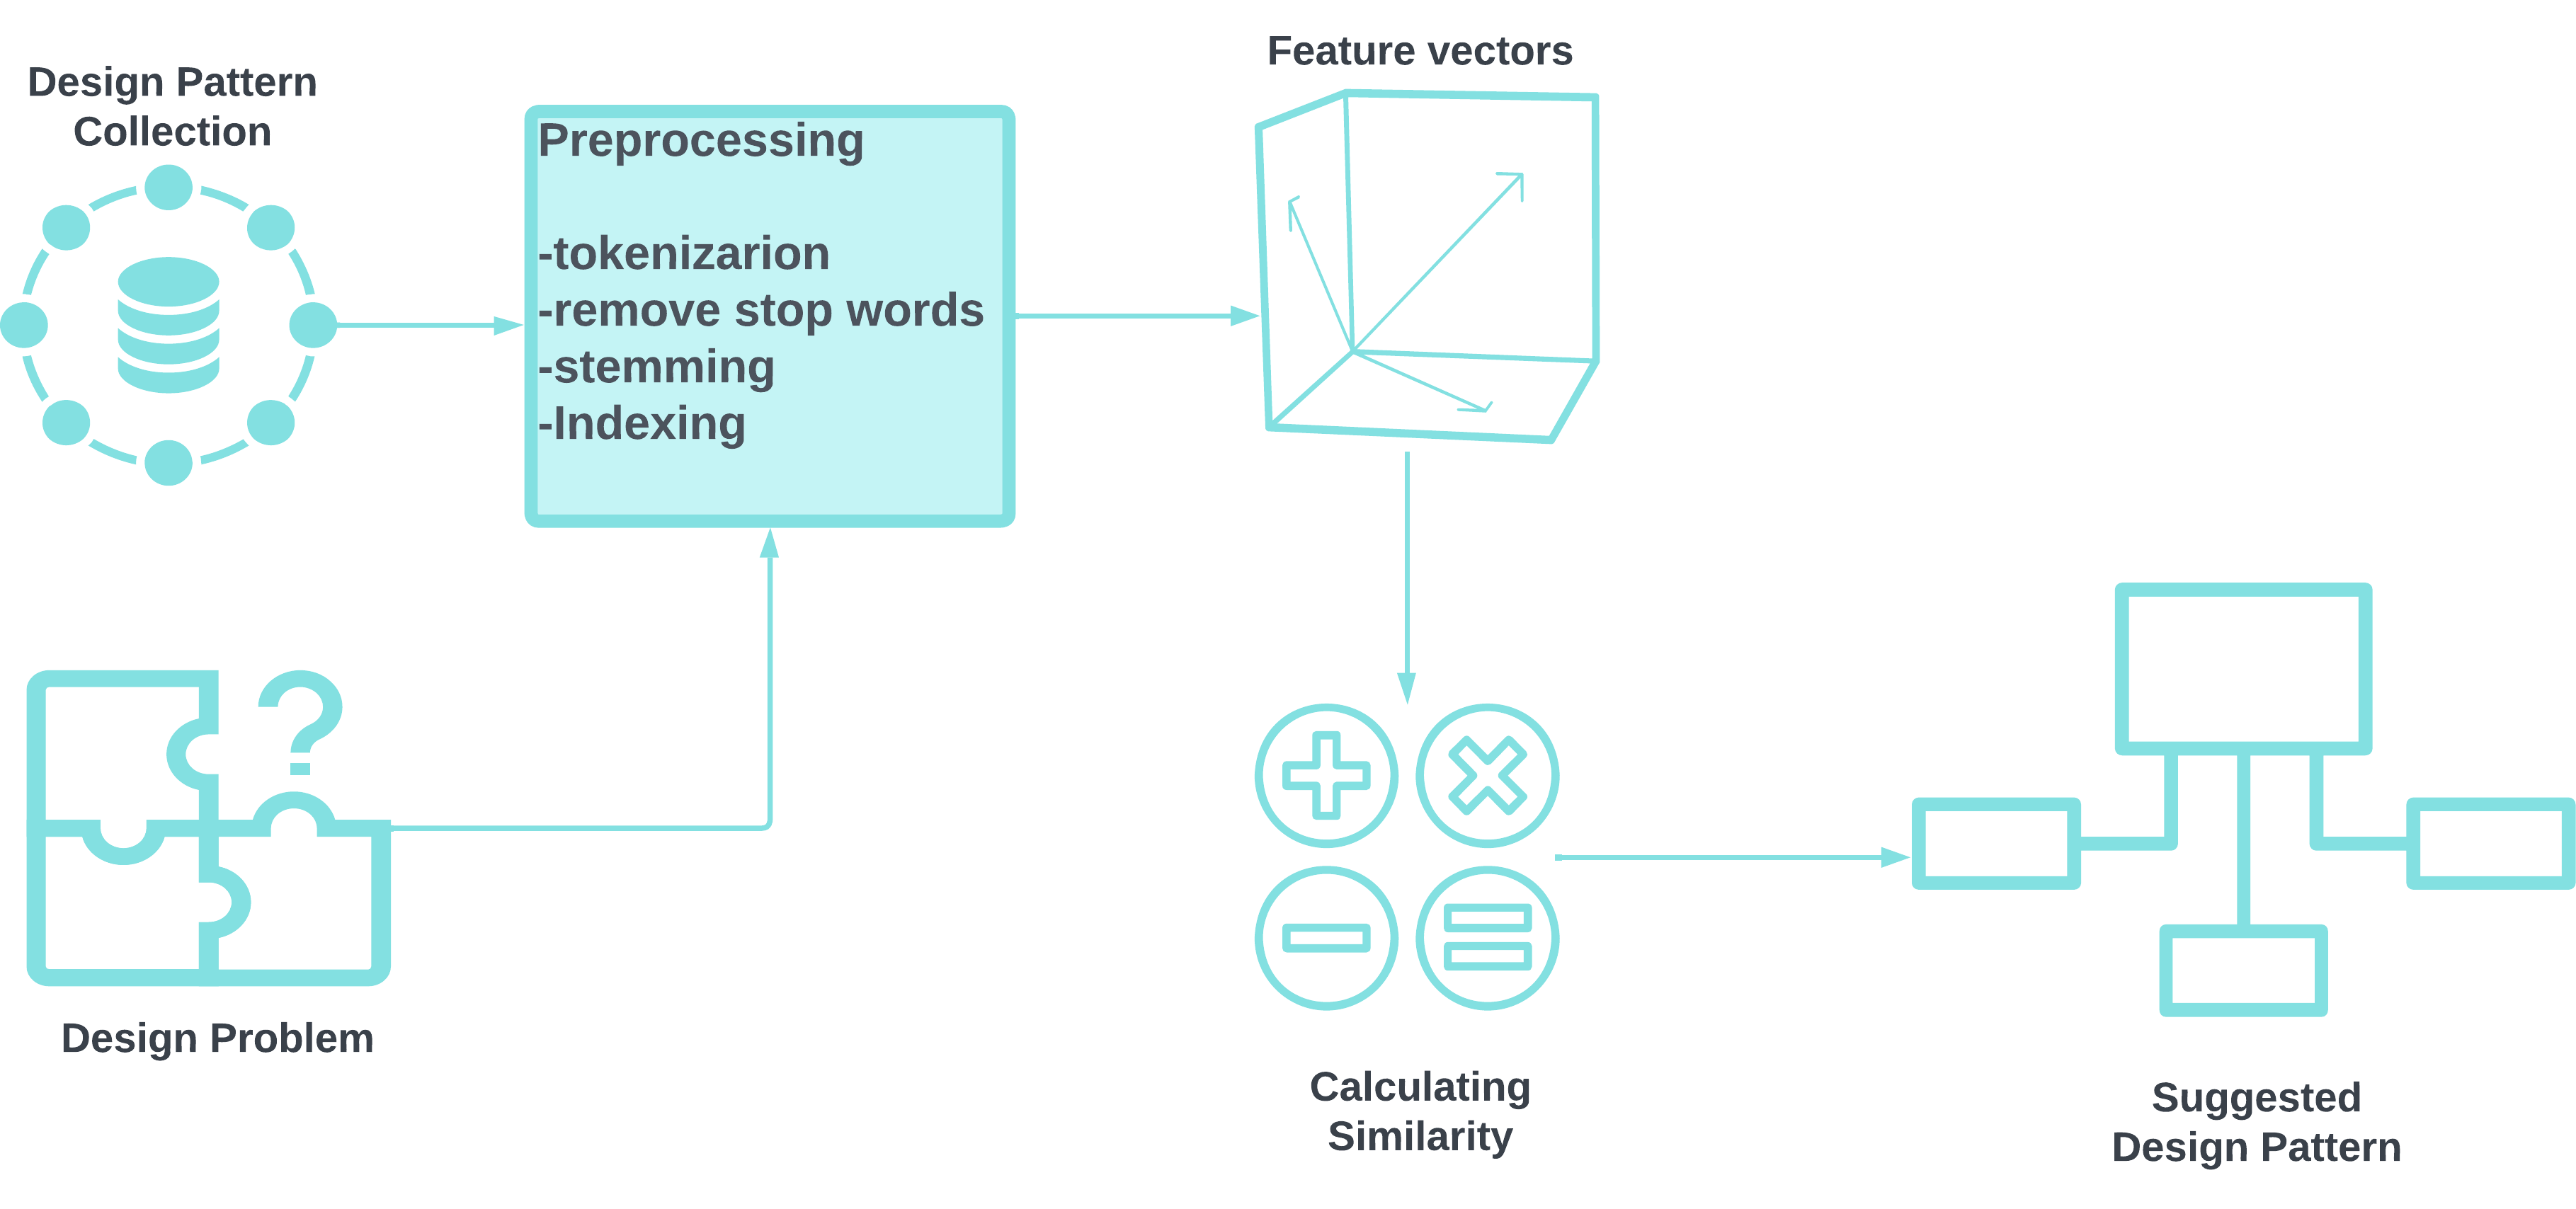
\includegraphics[width=0.9\textwidth]{figures/text-classification-retrieval-selected-pattern-approach.png}
\objectsource{\objectsourceauthor}
\end{figure}
% Fim Figura ---------------------------

First, the design patterns and problems are preliminarily prepared using data mining techniques to reduce feature set size and data sprawl. The pre-processing steps are tokenization, stop-word removal, stemming, and indexing. As a result, a feature vector is created for each design pattern and problem scenario. Term weighting techniques are used to improve the performance of the text retrieval process. The weight of each word indicates the term's relative importance in describing a given DP in the design pattern collection. Finally, a ranked list of design patterns for the given problem is retrieved using a similarity measure,~\textcite{Intakosum2007},~\textcite{Suresh2011},~\textcite{Hasheminejad2012},~\textcite{Sanyawong2015},~\textcite{Hamdy2018automatic},~\textcite{Rahmati2019} and~\textcite{ Jalil2020}  suggested suitable design patterns.

\textcite{Hamdy2018automatic} provided a method to suggest patterns based on the degree of similarity between design pattern vectors and design problem vectors. In this study, the authors created unigram and bigram features. Bigrams are essential for distinguishing between design patterns. However, the accuracy of this method is affected by an efficient dataset of design pattern descriptions and the quality of design problem scenarios.

Another method using the Latent Dirichlet Allocation (LDA) model to extract subject matter from pattern descriptions. A subject is a collection of words that usually appear together. Patterns are then suggested based on the similarity between the design pattern vector and the design problem vector~\cite{Hamdy2018Towards}.

\textcite{Suresh2011} used 26 case studies to evaluate a proposed framework for recommending design patterns that rely on two approaches: text retrieval and question-answer. This structure represents the design problem as a collection of words.

Initially, the system operates on this collection of query words to find a suitable design pattern whose intent is similar to the query words. In the next step, the intent of the top candidate design patterns is displayed for the designer to select the most suitable pattern intent. The system provides additional support to the designer by providing questions. The system scores the recommended standards based on the designer's responses. If no suitable candidate pattern is found, the system searches its history database for the most similar query. Then the matching pattern is allocated to the problem.

However, they have implemented and partially tested their framework. Also, using pattern intent only in the first step will yield poor performance and require user involvement in the selection process.

\MyPara{Ontology-Based Approach}\label{subsec:ontology-approach}

Ontology is very popular in computer science which enables domain knowledge to be modeled abstractly and enables queries to be evaluated against a knowledge base. There are various tools and methods to create an ontology domain. The Web Ontology Language (OWL) is a standard language for ontology representation whose primary syntax is XML/RDF (resource description framework) and is used to model knowledge of a particular domain. 

In modeling a domain using an ontology, all existing knowledge is modeled as a family of related concepts with interconnected relationships. One of the most important decisions in the ontology construction process is to select the appropriate ontology method, tools, and language. Manual and semi-automatic creation are the two methods of ontology construction used in the papers. Tools like Protégé~\textcite{Gennari2003} and Ontostudio~\textcite{Weiten2009} provide a suitable environment for the creation of ontology manually. This method of ontology construction often does not use data mining tools.

In contrast, human intervention is reduced in the semi-automatic creation method, and the speed of ontology construction and development is increased. Tools like text2onto~\textcite{Cimiano2005} and Ontolearn~\textcite{Velardi2013} use machine-learning techniques to create an ontology. These tools usually require a large sample for training. 

The existing studies for selecting a design pattern based on the ontology approach concluded that the pattern suggestion process in this approach is as shown in Figure~\ref{fig-ontology-base-approach}. As shown in this figure, the principal and typical phase in the ontology-based approach is constructing an ontology of the concepts in the pattern description.

% Inicio Figura ---------------------------
\begin{figure}[ht]
\caption{Overview of ontological approach for analysis patterns.}
\centering
\label{fig-ontology-base-approach}
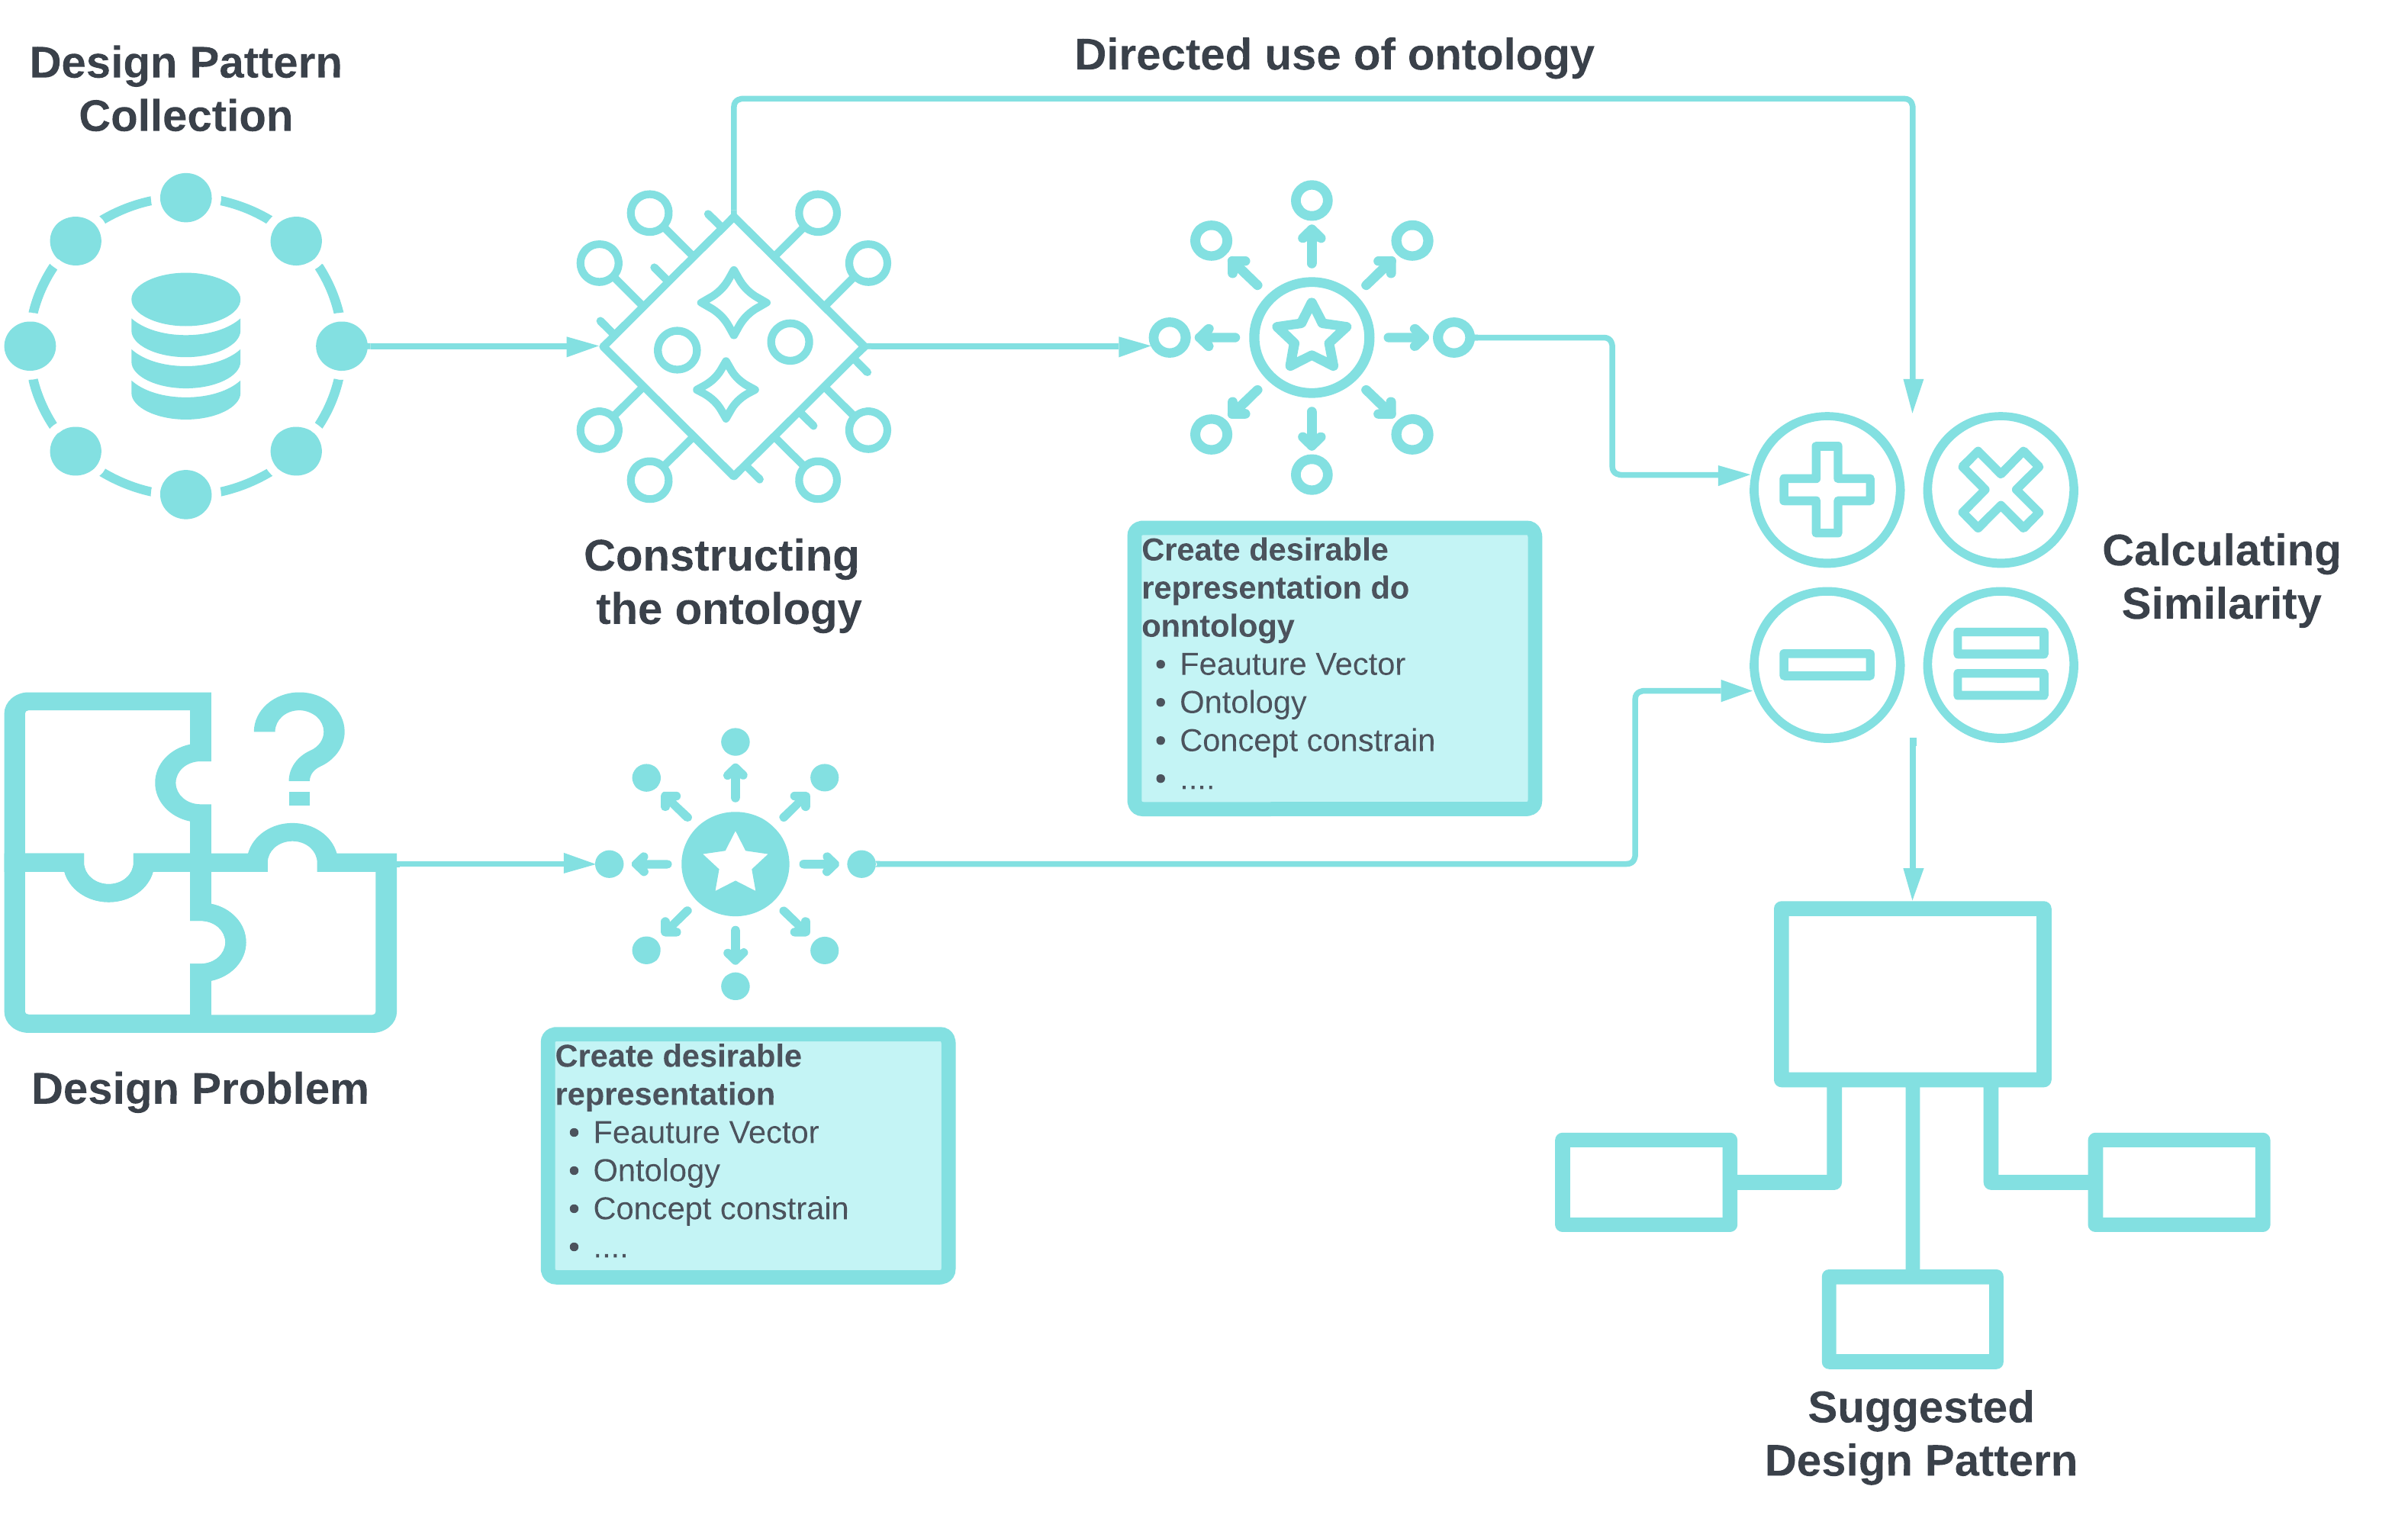
\includegraphics[width=1.0\textwidth]{figures/ontology-base-selected-pattern-approach.png}
\objectsource{\objectsourceauthor}
\end{figure}
% Fim Figura ---------------------------

\textcite{Hamza2004, El2008, Di2014, Sielis2017, Naghdipour2021} have suggested suitable design patterns. There are different methods to use the constructed ontology to suggest the pattern. For instance,~\textcite{Kampffmeyer2007} provided a wizard that enables the designer to enter their problem and find the design patterns from constructed ontology.

However, the designer can only use the concepts defined in the ontology.~\textcite{Bou2018} preprocessed the constructed ontology and the design problem to create feature vectors. They suggested design patterns based on the similarity between design patterns and design problem vectors.~\textcite{Blomqvist2008} created an ontology for the design problem and tried to find the similarity between the constructed ontology from patterns and problems.


 \MyPara{Others Approaches}\label{subsec:others-approach}
 
In addition to the mentioned approaches, some researchers have employed alternative methods, known as other approaches, to suggest suitable design patterns~\cite{Zdun2007, Pearson2010, Pearson2010}. 

\textcite{Zdun2007} proposed a two-step approach considering desired quality attributes and pattern relations. Firstly, they formalized pattern relationships using a pattern language grammar annotated with effects on quality goals. This allowed for the automatic derivation of pattern sequences from the grammar, and the quality goal annotations provided an approximate overview of the impact of design decisions on quality goals. Secondly, they utilized design spaces to analyze design decisions, enabling the generation of a detailed decision map.

\textcite{Bouassida2011} developed a tool that recommends the appropriate design pattern from a pattern repository and assists in instantiating the chosen pattern. Their approach utilizes a set of comparison criteria and creates rules for pattern recommendation. In the first step, the user's design fragment is analyzed using various semantic criteria, generating an XML file to identify the most suitable solution. In the second step, they employ forty rules based on semantic comparison criteria to recommend and instantiate the design patterns.


\MyPara{Combination of Approaches:}\label{subsec:combination-approach}


It is worth mentioning that certain articles have employed a blend of various methods. Board \ref{board:combined-approach} exhibits the approach combinations utilized in diverse studies and their references. The combination of QA, CBR, and IR is the most commonly employed.
 
\begin{table}[ht]
    \centering
    \footnotesize
    \setlength{\tabcolsep}{4pt}
    \board{Types of the combination of the design patterns selection approaches}
    \label{board:combined-approach}
    \begin{tabular}{|l|p{.60\linewidth}|r|p{.01\linewidth}|} \hline
        \rowcolor{gray!19} \textbf{Approaches Category} & \textbf{References} \\ \hline
        Ontology and IR & \textcite{Bou2018, Laosen2020} \\
        \rowcolor{gray!19} Ontology and CBR & \textcite{Blomqvist2008} \\ 
        Ontology and QA & \textcite{Pavlivc2014} \\
        \rowcolor{gray!19} CBR and IR & \textcite{Muangon2009adaptation,Muangon2009analysis} \\ 
        CBR and QA & \textcite{Qureshi2017} \\
        \rowcolor{gray!19} CBR, QA and IR & \textcite{Sanyawong2014,Bouassida2015, Celikkan2019} \\ \hline 
    \end{tabular}
    \objectsource{\objectsourceauthor}
\end{table}
  
\MyPara{Trade-offs between the Design Patterns Selection Approaches} \label{subsec:trade-offs-approaches}

\textcite{Kim2007} presented a UML-based method that utilizes Role-Based Modeling Language (RBML) to create the meta-model for each pattern and problem. They used collaboration and class diagrams to specify different aspects of patterns, resulting in different properties, such as structural and behavioral. Finally, if the design pattern's specifications can meet the problem's diagram, a pattern is suggested. However, the method's scalability could be improved due to overlapping meta-models.

\textcite{Muangon2013} presented a CBR-based method that uses formal concept analysis (FCA) to solve the problem of design pattern retrieval caused by differences between author and user keywords. A similarity function retrieves similar cases for the input problem in their proposed method. FCA is used to reformulate problem descriptions and retrieve related cases if the user is unsatisfied with the proposed pattern. The quality and variety of the case base can affect the accuracy of pattern suggestion, and finding similarities between the previous problems and the new problem can be time-consuming.

\textcite{Nahar2016} analyzed anti-patterns corresponding to the design patterns to identify the structural, behavioral, and semantic properties. These three levels of analysis are performed to capture anti-pattern information accurately. Scores are assigned to design patterns based on analysis and matching, and the highest-scoring pattern is proposed for a given design problem. However, the method requires a logical description of these anti-patterns.

\textcite{Qureshi2017} proposed a Q-A-based design pattern selection model that provides questions based on the design patterns' properties. After interacting with the user, the answers are weighted, and the design pattern with the highest weight (similarity) is suggested to the designer. Providing the questions is the main challenge of this study.

\textcite{Hussain2017software} proposed a three-phase method to automate the selection of design patterns. In the first phase, the problem part of the pattern description and the design problem are pre-processed to create their weighted vectors. In the second phase, the classifiers are trained on feature vectors using the "LambdaMART" algorithm, a supervised learning technique. In the last phase, the suitable patterns are retrieved for a given design problem using similarity measurements. The classifier's performance is influenced by sample size and ranking algorithms.

\textcite{Hamdy2018automatic, Hamdy2018Towards} presented a two-phase IR-based method to suggest design patterns. In the first phase, data mining techniques are used to pre-process the set of design patterns and design problems to reduce the feature set's size and the dataset's sparsity. In the second phase, the similarity between patterns and problem vectors is calculated, and a ranked list of design patterns for the given problem is retrieved. Efficient descriptions of design patterns and design problem scenarios influence the accuracy of the proposed method.

\textcite{Hussain2019automated} presented a text classification-based method using the Fuzzy c-means algorithm, an unsupervised learning algorithm, to automate the design pattern selection process. However, the multi-class problem is the method's shortcoming. Additionally, the Fuzzy c-mean algorithm is the only algorithm used to learn all the datasets, while choosing the suitable clustering or classification algorithm depends on the problem context.

\textcite{Naghdipour2021} manually created an ontology and connected it to WordNet to suggest a more accurate design pattern. However, manually constructing an ontology is costly and requires professional work.

\textcite{Naghdipour2023Semi} proposes an evaluation model using three widely used case studies and 109 real design problems. design to assess its effectiveness. The evaluation results indicate that the proposed method's performance has improved compared to the supervised learning techniques of Naïve Bayes and KNearestNeighbor.

The field of design pattern selection still faces several major issues that need to be addressed for further development. One common issue is the evaluation of methodologies on small datasets. Many papers use a limited number of real design problems or gather feedback from only a few users to evaluate their methods. This limited evaluation scope raises concerns about the applicability and correctness of the proposed design patterns in larger and more complex cases. Methods must be tested and confirmed to work effectively in large and real-world scenarios~\cite{Naghdipour2023}.

Another issue is the reliance on a narrow collection of design patterns in implementing methods. Most proposed methods focus solely on the Gang of Four (GoF) design pattern collection, and some are limited to specific categories or subsets of design patterns~\cite{Schumacher2013}. This issue can be addressed by using suitable input types and expanding the collections of design patterns used in research. It is essential to ensure that the input types adequately support the functionality required by the proposed methods and encompass a broader range of design patterns, including patterns beyond the GoF collection.

Semi-automatic methods that require interaction with developers or designers are also a limitation. The ideal approach would be fully automated, allowing large-scale applications without manual intervention. To achieve this, techniques such as text mining, clustering, \ac{ML}, and \ac{AI} can be employed. These automated techniques can handle large amounts of data and accelerate implementation. The goal is to improve efficiency and accuracy in pattern suggestion by exploring different methods and algorithms related to these techniques~\cite {Naghdipour2023}.

Despite the advances in design pattern selection, there are still concerns regarding the focus on specific patterns and issues related to cost, time, comprehensiveness, and the evaluation of methods. These areas require further improvement and exploration to enhance the effectiveness and practicality of design pattern selection approaches. 

\section{Architecture Decision-Making}\label{sec:architecture-decision-making}

% The state of the art on design patterns: A systematic mapping of the literature \cite{Mayvan2017}
% \subsection{LLMs Design Patterns}
% \subsection{Architectural Design Patterns} \cite{Taibi2018}
% \subsection{LLM Prompt Design Patterns}
